\documentclass[14pt, a4paper]{report}
\usepackage{mathtext}
\usepackage[T2A]{fontenc}
\usepackage[utf8]{inputenc}
\usepackage[russian]{babel}
\usepackage{multirow}
\usepackage{slashbox}
\usepackage{makecell}
\usepackage{graphicx}
\usepackage{physics}
\usepackage{amstext}
\usepackage{caption}
\usepackage{subcaption}
\usepackage{cmap}
\usepackage{float}
\usepackage{indentfirst}
\usepackage{romannum}

\usepackage[a4paper,
            		left=1in,
            		right=1in,
           		 top=1in,
            		bottom=1in,
            		footskip=.25in]{geometry}

\renewcommand{\thesection}{\arabic{section}.}
\renewcommand{\thesubsection}{\arabic{section}.\arabic{subsection}.}

\title{\textbf{Отчет о выполнении лабораторной работы 5.10.1 "Электронный парамагнитный резонанс"}}
\author{Калашников Михаил, Б03-202}
\date{}

\begin{document}
\maketitle

\pagenumbering{arabic}

\section{Теоретические сведения}

Явление электронного парамагнитного резонанса (ЭПР) было открыто советским физиком Е.К. Завойским в 1943 году. К настоящему времени этот метод получил большое развитие и применяется как в исследованиях в области физики, так и в химических и биологических приложениях. В данной лабораторной работе мы изучаем простейшую постановку ЭПР эксперимента.
В методе ЭПР изучается резонансное поглощение переменного электромагнитного поля в образце в зависимости от контролируемых экспериментатором внешних условий: постоянного магнитного поля, частоты колебаний переменного поля, температуры и так далее.

Простейшей моделью для рассмотрения ЭПР является система из невзаимодействующих частиц со спином $S=1/2$, помещённая во внешнее магнитное поле. В отсутствие магнитного поля энергии состояний с проекцией спина $S_z=\pm1/2$ совпадают. Из-за эффекта Зеемана энергии состояний с различными проекциями спина начинают различаться. Если направить на нашу систему поток излучения (поток фотонов) с энергией,
равной разнице энергий этих состояний $h\nu=g\mu_B B$, то станут возможны индуцированные переходы между состояниями. Эти переходы происходят с поглощением или испусканием фотона в зависимости от того, в каком из состояний была система до взаимодействия с излучением.

\begin{figure}[H]
\centering
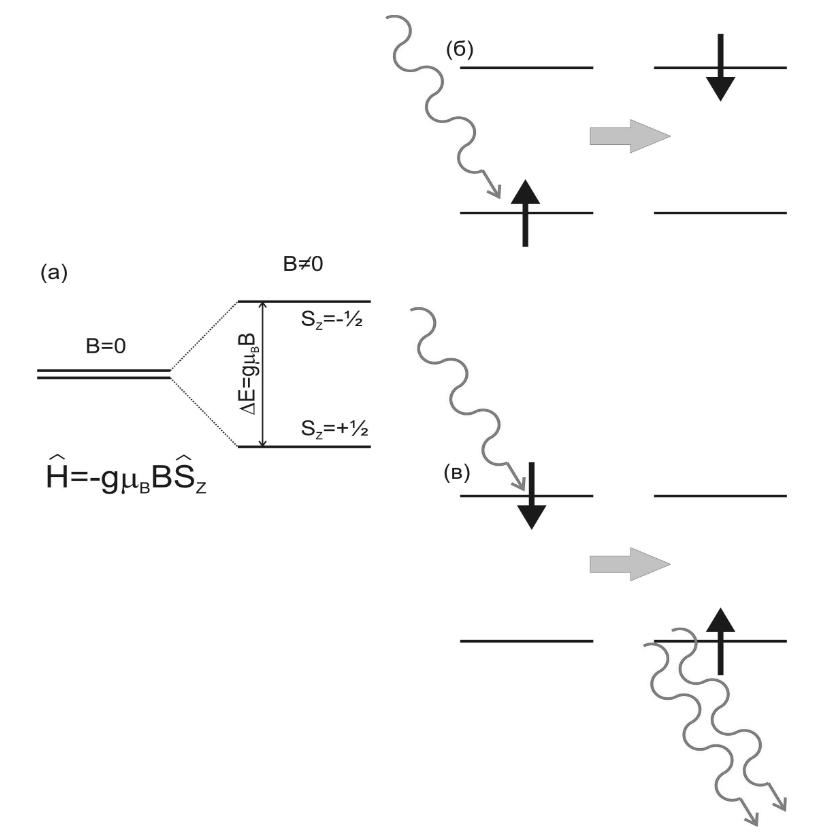
\includegraphics[width=.8\linewidth]{../images/5101-2}
\caption{Схема резонансного поглощения электромагнитного излучения для изолированного спина $S=1/2$. (a) Зеемановское расщепление спинового уровня в магнитном поле. (б) Переход между подуровнями «снизу-вверх» с поглощением фотона резонансной частоты $h\nu=g\mu_B B$. (в) Переход между подуровнями «сверху-вниз» с излучением дополнительного фотона резонансной частоты.}
\end{figure}

\section{Экспериментальная установка}

В работе исследуется ЭПР в дифенилпикрилгидразиле, сокращённо обозначаемом ДФПГ. В твёрдом состоянии молекулы ДФПГ формируют молекулярный кристалл. Исследуемый образец состоит из некоторого количества порошка твёрдого ДФПГ, помещённого в стеклянную ампулу. Один из электронов центрального атома азота остаётся неспаренным, резонансное поглощение наблюдается именно на этом электроне.

\begin{figure}[H]
\centering
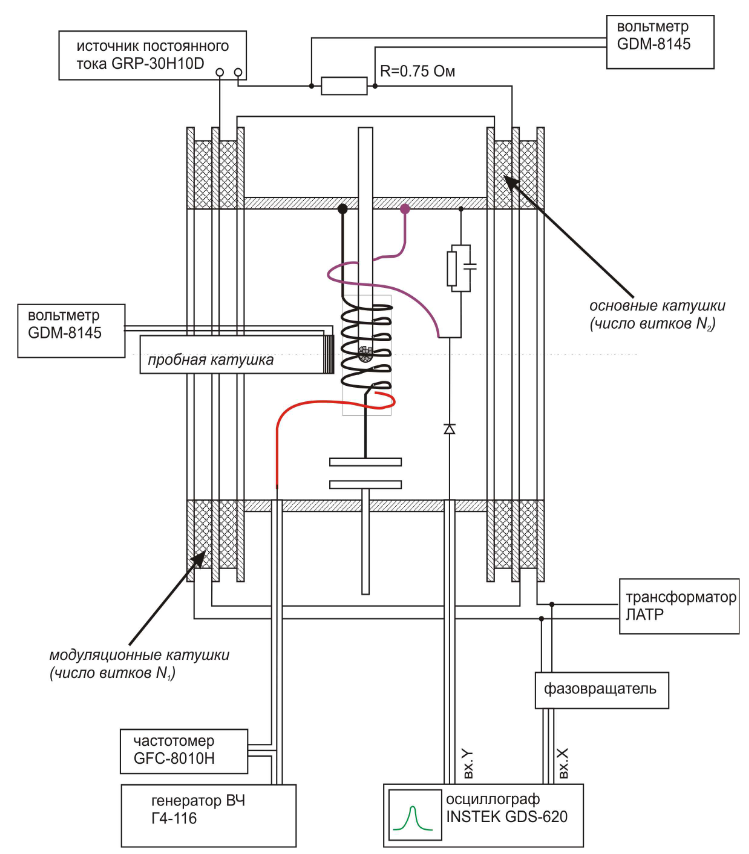
\includegraphics[width=.8\linewidth]{../images/5101-3}
\caption{Схема установки}
\end{figure}

Схема установки показана на рисунке выше. Переменное электромагнитное поле на частоте ~100 МГц создаётся высокочастотным генератором, постоянное магнитное поле создаётся электромагнитом. Для увеличения чувствительности эксперимента образец помещают в катушку индуктивности колебательного контура. Колебательный контур состоит из катушки индуктивности и плоского конденсатора. Ёмкость конденсатора может изменяться подстройкой расстояния между пластинами при помощи штока.

Для создания магнитного поля используется электромагнит, состоящий из пары разнесённых катушек. Ток через электромагнит контролируется по падению напряжения на резисторе, включённом в цепь питания катушек. Дополнительно к основным катушкам имеется пара модуляционных катушек, в которые могут создавать переменное поле малой амплитуды. Для создания переменного поля к катушкам прикладывается напряжение с трансформатора ЛАТР, частота колебаний переменного поля соответствует частоте колебаний напряжения в сети переменного тока.

\section{Проведение эксперимента и обработка результатов}

\subsection{Настройка ВЧ генератора}

\begin{enumerate}

\item Настроим ВЧ генератора на частоту колебательного контура. Переведем ВЧ генератор в режим амплитудной модуляции, установим глубину модуляции равной 10\%. Подстройкой частоты генератора добьемся максимальной амплитуды сигнала на экране осциллографа.
\[f_0=(130.3\pm0.1)\ МГц\]

\item Добротность колебательного контура может быть определена по расстройке частоты до достижения сигналом половины от максимального достижения в сторону больших и маленьких частот.
\[f_{+\frac{1}{2}}=(131.1\pm0.1)\ МГц\quad f_{-\frac{1}{2}}=(129.7\pm0.1)\ МГц\]

\[Q=\frac{f_0}{f_{+\frac{1}{2}}-f_{-\frac{1}{2}}}=93\pm9\]

\end{enumerate}

\subsection{Наблюдение сигнала резонансного поглощения}

\begin{enumerate}

\item Подключим основные катушки к трансформатору ЛАТР. Осциллограф оставим в режиме развертки по времени. Подадим на модуляционные катушки напряжение ~50 В. 

\item Плавно будем увеличивать напряжение, подаваемое на основные катушки до появлении на экране осциллографа картины резонансного поглощения.

\item Добившись максимально точно настройки постоянного поля на резонансное поглощение, сфотографируем наблюдаемую картину.

\begin{figure}[H]
\centering
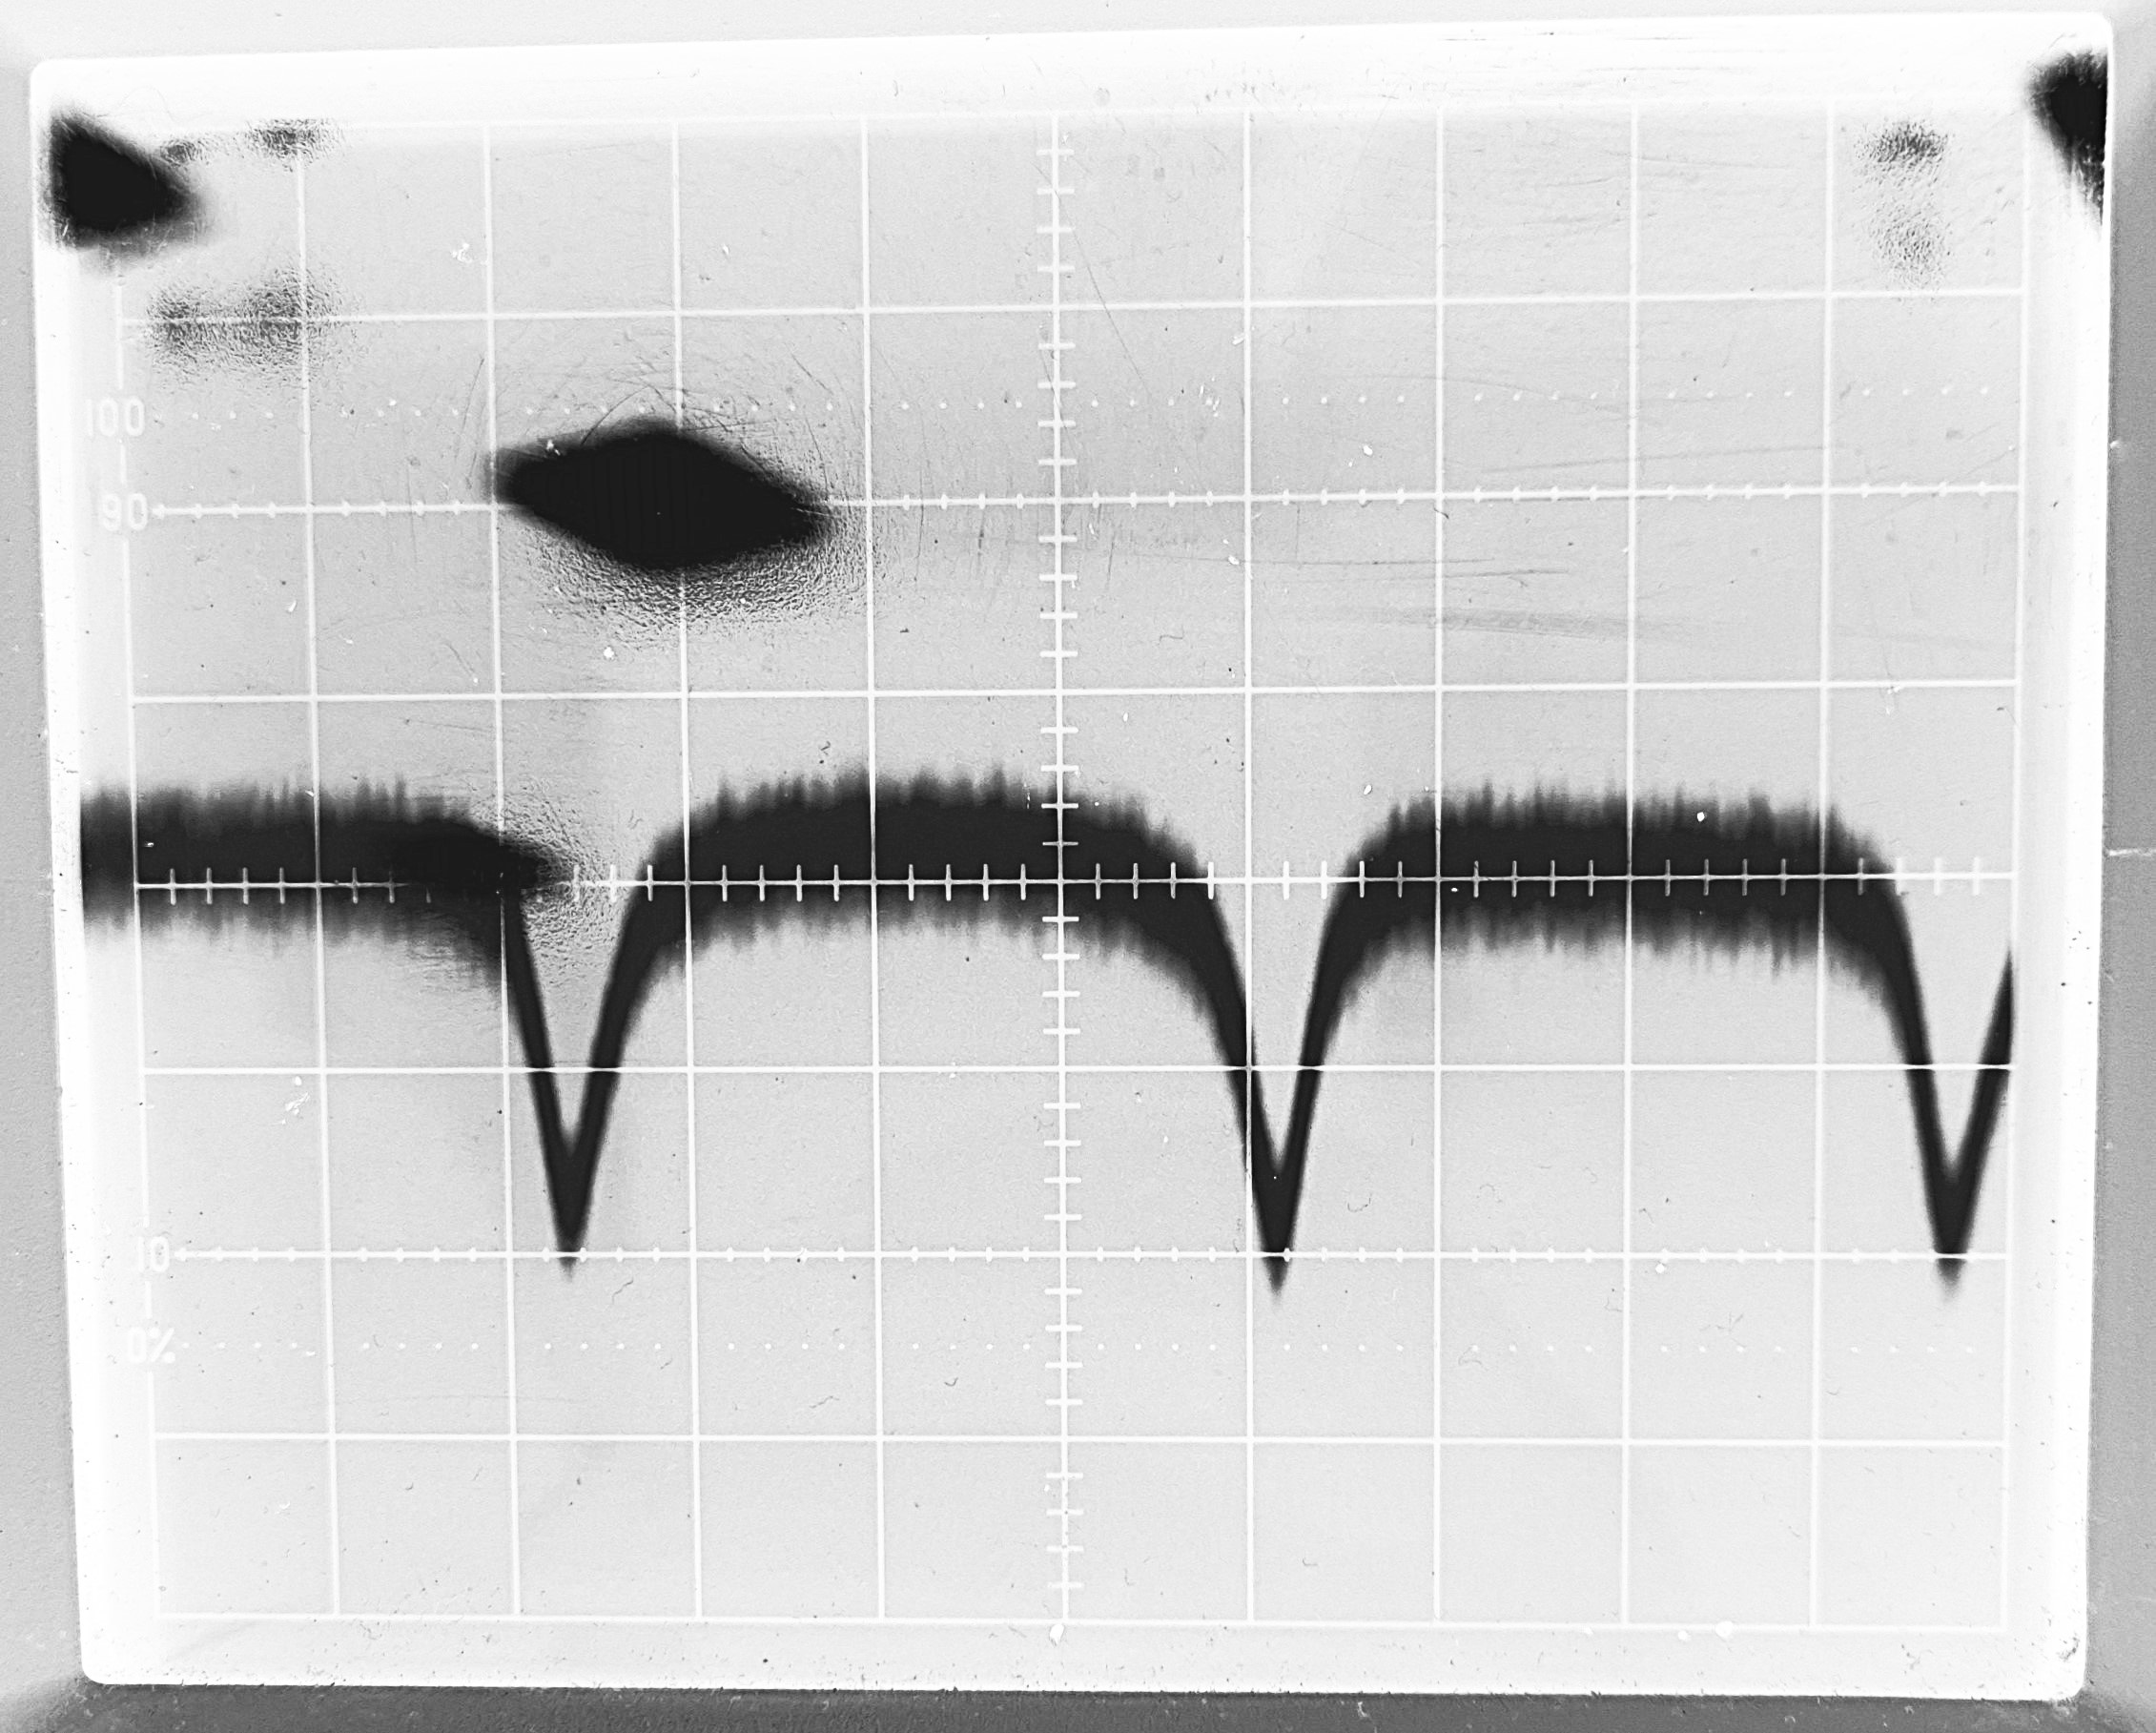
\includegraphics[width=.8\linewidth]{../images/5101-4}
\caption{Сигнал резонансного поглощения на экране осциллографа}
\end{figure}

\end{enumerate}

\subsection{Точная настройка резонансного поля и определение ширины линии}

\begin{enumerate}

\item Для более точной настройки и определения ширины линии резонансного поглощения подадим на X-сигнал осциллографа напряжение, прикладываемое к модуляционным катушкам и пронаблюдаем сигнал в XY-режиме. Точной настройкой постоянного поля и подстройкой фазовращателся добьемся симметрии картины относительно средней вертикальной оси. При этом падение напряжения на резисторе в цепи основных катушек составит
\[U_0=(64.3\pm4.4)\ мВ\]

\begin{figure}[H]
\centering
\begin{subfigure}{.5\textwidth}
  \centering
  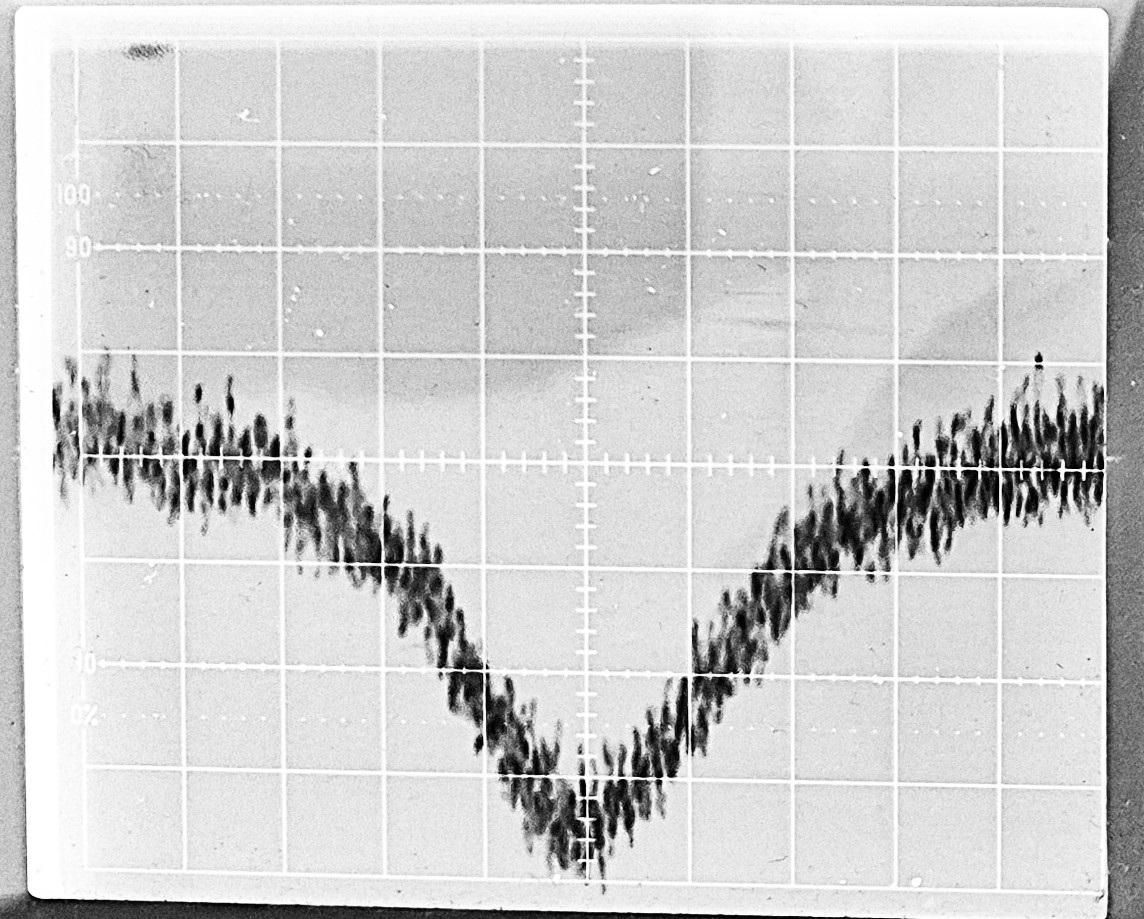
\includegraphics[width=.9\linewidth]{../images/5101-5}
  \caption{Точная настройка резонансного поля}
\end{subfigure}%
\begin{subfigure}{.5\textwidth}
  \centering
  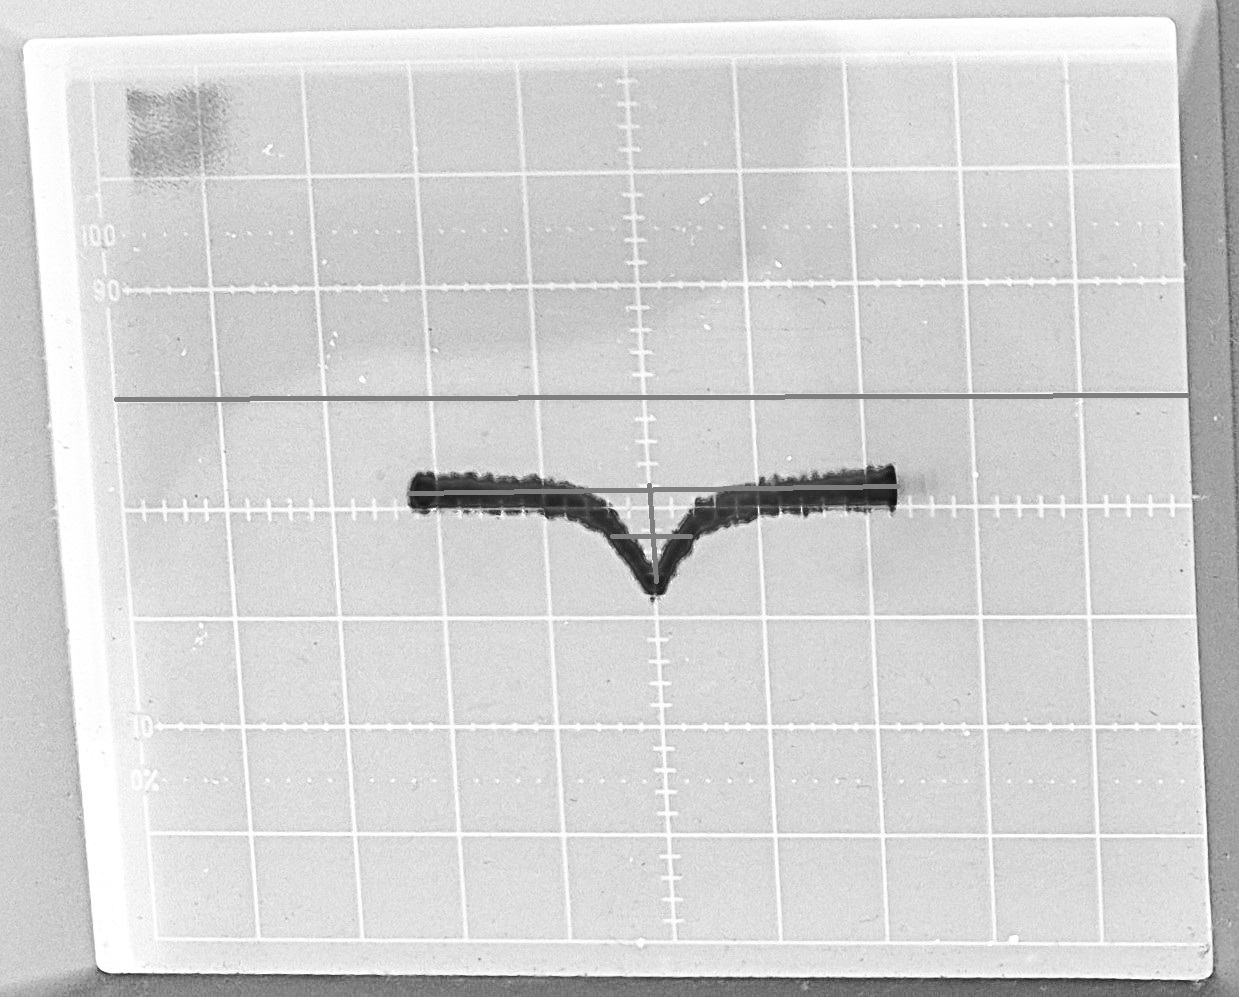
\includegraphics[width=.9\linewidth]{../images/5101-6}
  \caption{Определение ширины линии ЭПР}
\end{subfigure}
\end{figure}

\item Для определения ширины линии ЭПР определим по экрасну осциллографа полный размах модулируещего поля $A_{полн}$ и полную ширину кривой резонансного поглощения на полувысоте $A_{1/2}$.
\[A_{полн}=(4.59\pm 0.10)\ дел.\quad A_{1/2}=(0.74\pm0.09)\ дел.\]

\item Внесем пробную катушку ($N_{проб}=46$, $d=(14.6\pm0.1)\ мм$) внутрь соленоида максимально близко к образцу. Зафиксируем показания вольтметра. $\varepsilon=2.65\ мВ$ Амплитуду модулирующего поля и полуширину на полувысоте линии резонансного поглощения можно определить по формулам
\[B_{мод}=\sqrt{2}\frac{2\varepsilon}{\pi^2 d^2 N_{проб} \nu}=(1.54\pm0.03)\ мТл\]
\[\Delta B=\frac{A_{1/2}}{A_{полн}}B_{мод}=(0.25\pm0.03)\ мТл\]

\end{enumerate}

\subsection{Калибровка поля электромагнита и определение g-фактора}

\begin{enumerate}

\item Для проведения калибровочных измерений переключим основные катушки на ЛАТР. Установим ток через катушки близкий к значению тока при наблюдении резонансного поглощения и измерим в этих условиях ЭДС индукции в пробной катушке.

\item Для повышения точности проведем калибровочные измерения при нескольких значениях тока. Также будем вносить катушку с передней и задней сторон установки.

\item Построим график зависимости ЭДС индукции в пробной катушке от напряжения на резисторе в цепи основных катушек.

\begin{figure}[H]
\centering
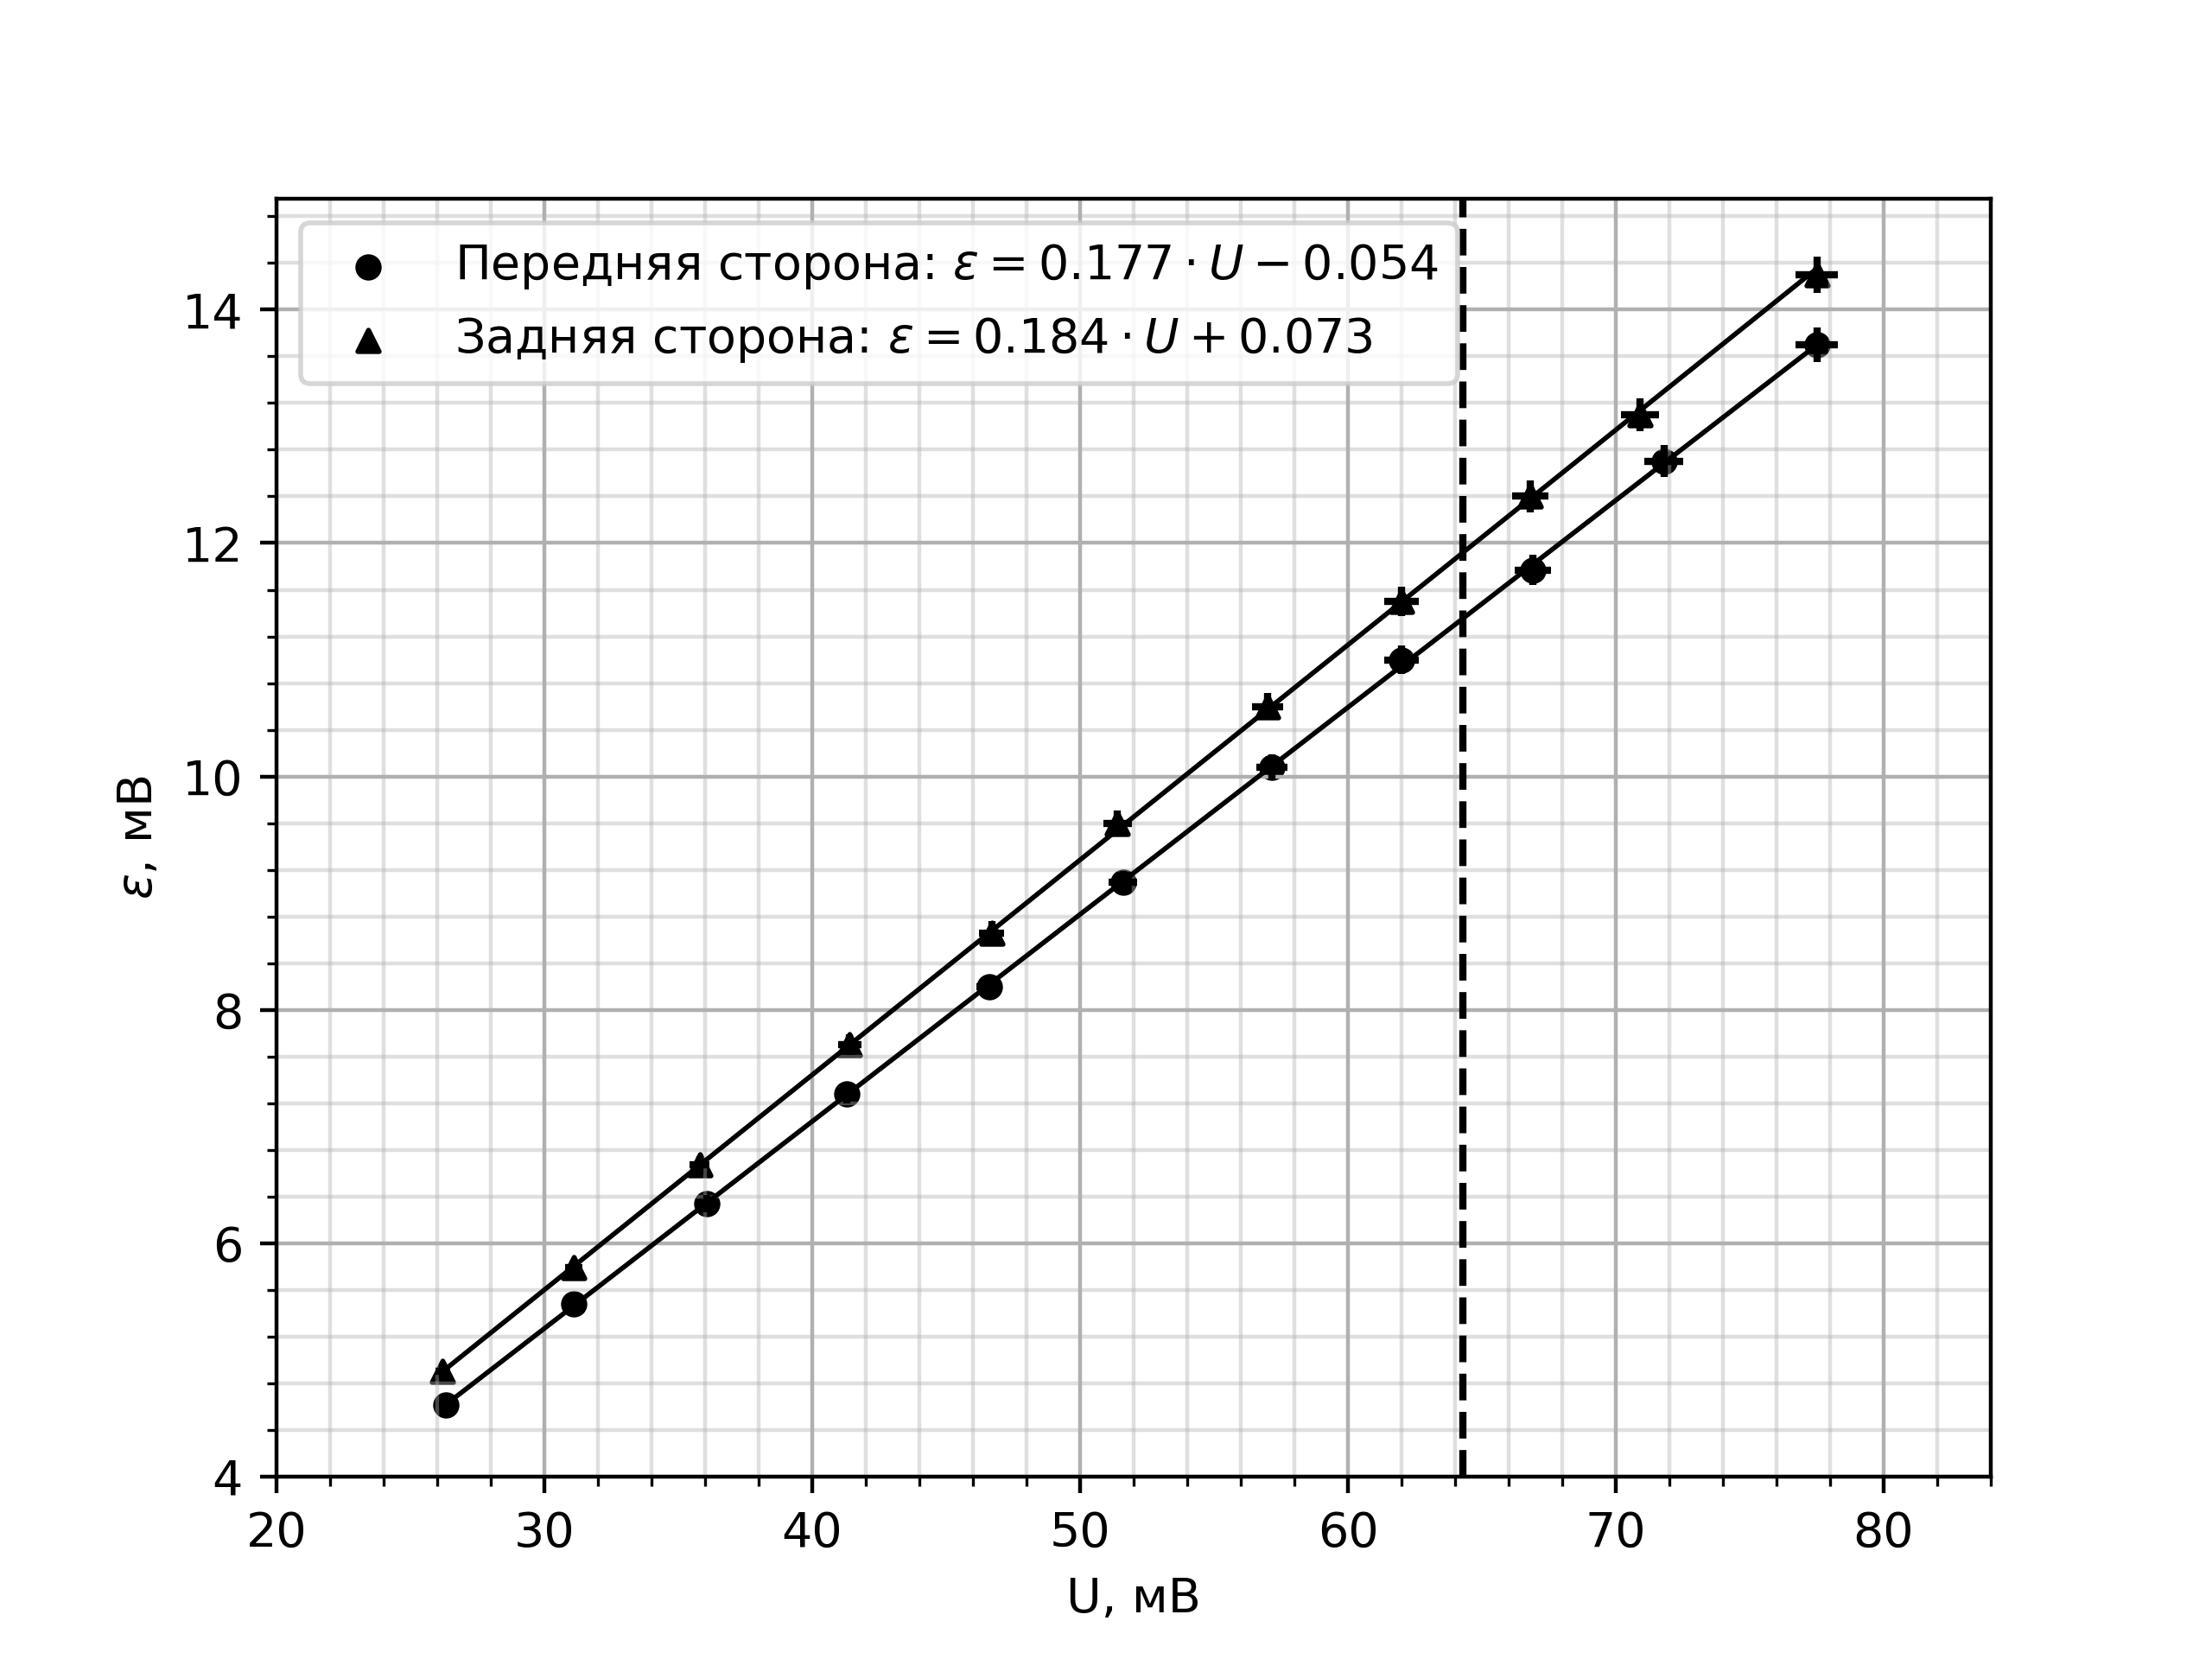
\includegraphics[width=.8\linewidth]{../images/5101-1}
\caption{Зависимость ЭДС индукции в пробной катушке от напряжения на резисторе в цепи основных катушек}
\end{figure}

\item Рассмотрим прямые, проведенные через экспериментальные точки, как калибровочные прямые. По ним определим ЭДС индукции при падении напряжения, необходимом для наблюдения резонансного поглощения ($U_0=(64.3\pm4.4)\ мВ$).
\[\varepsilon_1=(11.4\pm0.8)\ мВ,\quad \varepsilon_2=(11.9\pm0.8)\ мВ\]

\item Рассчитаем поле у передней и задней сторон установки по формуле 
\[B=\frac{2\varepsilon}{\pi^2 d^2 N_{проб} \nu}\]
\[B_1=(4.7\pm0.3)\ мТл,\quad B_2=(4.9\pm0.2)\ мТл\]
Для определение g-фактора возьмем среднее поле:
\[B_0=\frac{B_1+B_2}{2}=(4.8\pm0.2)\ мТл\]

\item g-фактор определим из условия возникновения электронного парамагнитного резонанса:
\[g\mu_B B_0=h\nu\]
\[g=\frac{h\nu}{\mu_B B_0}=1.94\pm0.10\]

\end{enumerate}

\newpage

\subsection{Измерение на нескольких частотах}

\begin{enumerate}

\item В ходе данного эксперимента будем изменять величину зазора конденсатора и тем самым менять резонансную частоту колебательного контура. При этом ток, подаваемый на основные катушки, менять не будем. Для пяти различных значений резонансной частоты сфотографируем экран осциллографа.

\begin{figure}[H]
\centering
\begin{subfigure}{.5\textwidth}
  \centering
  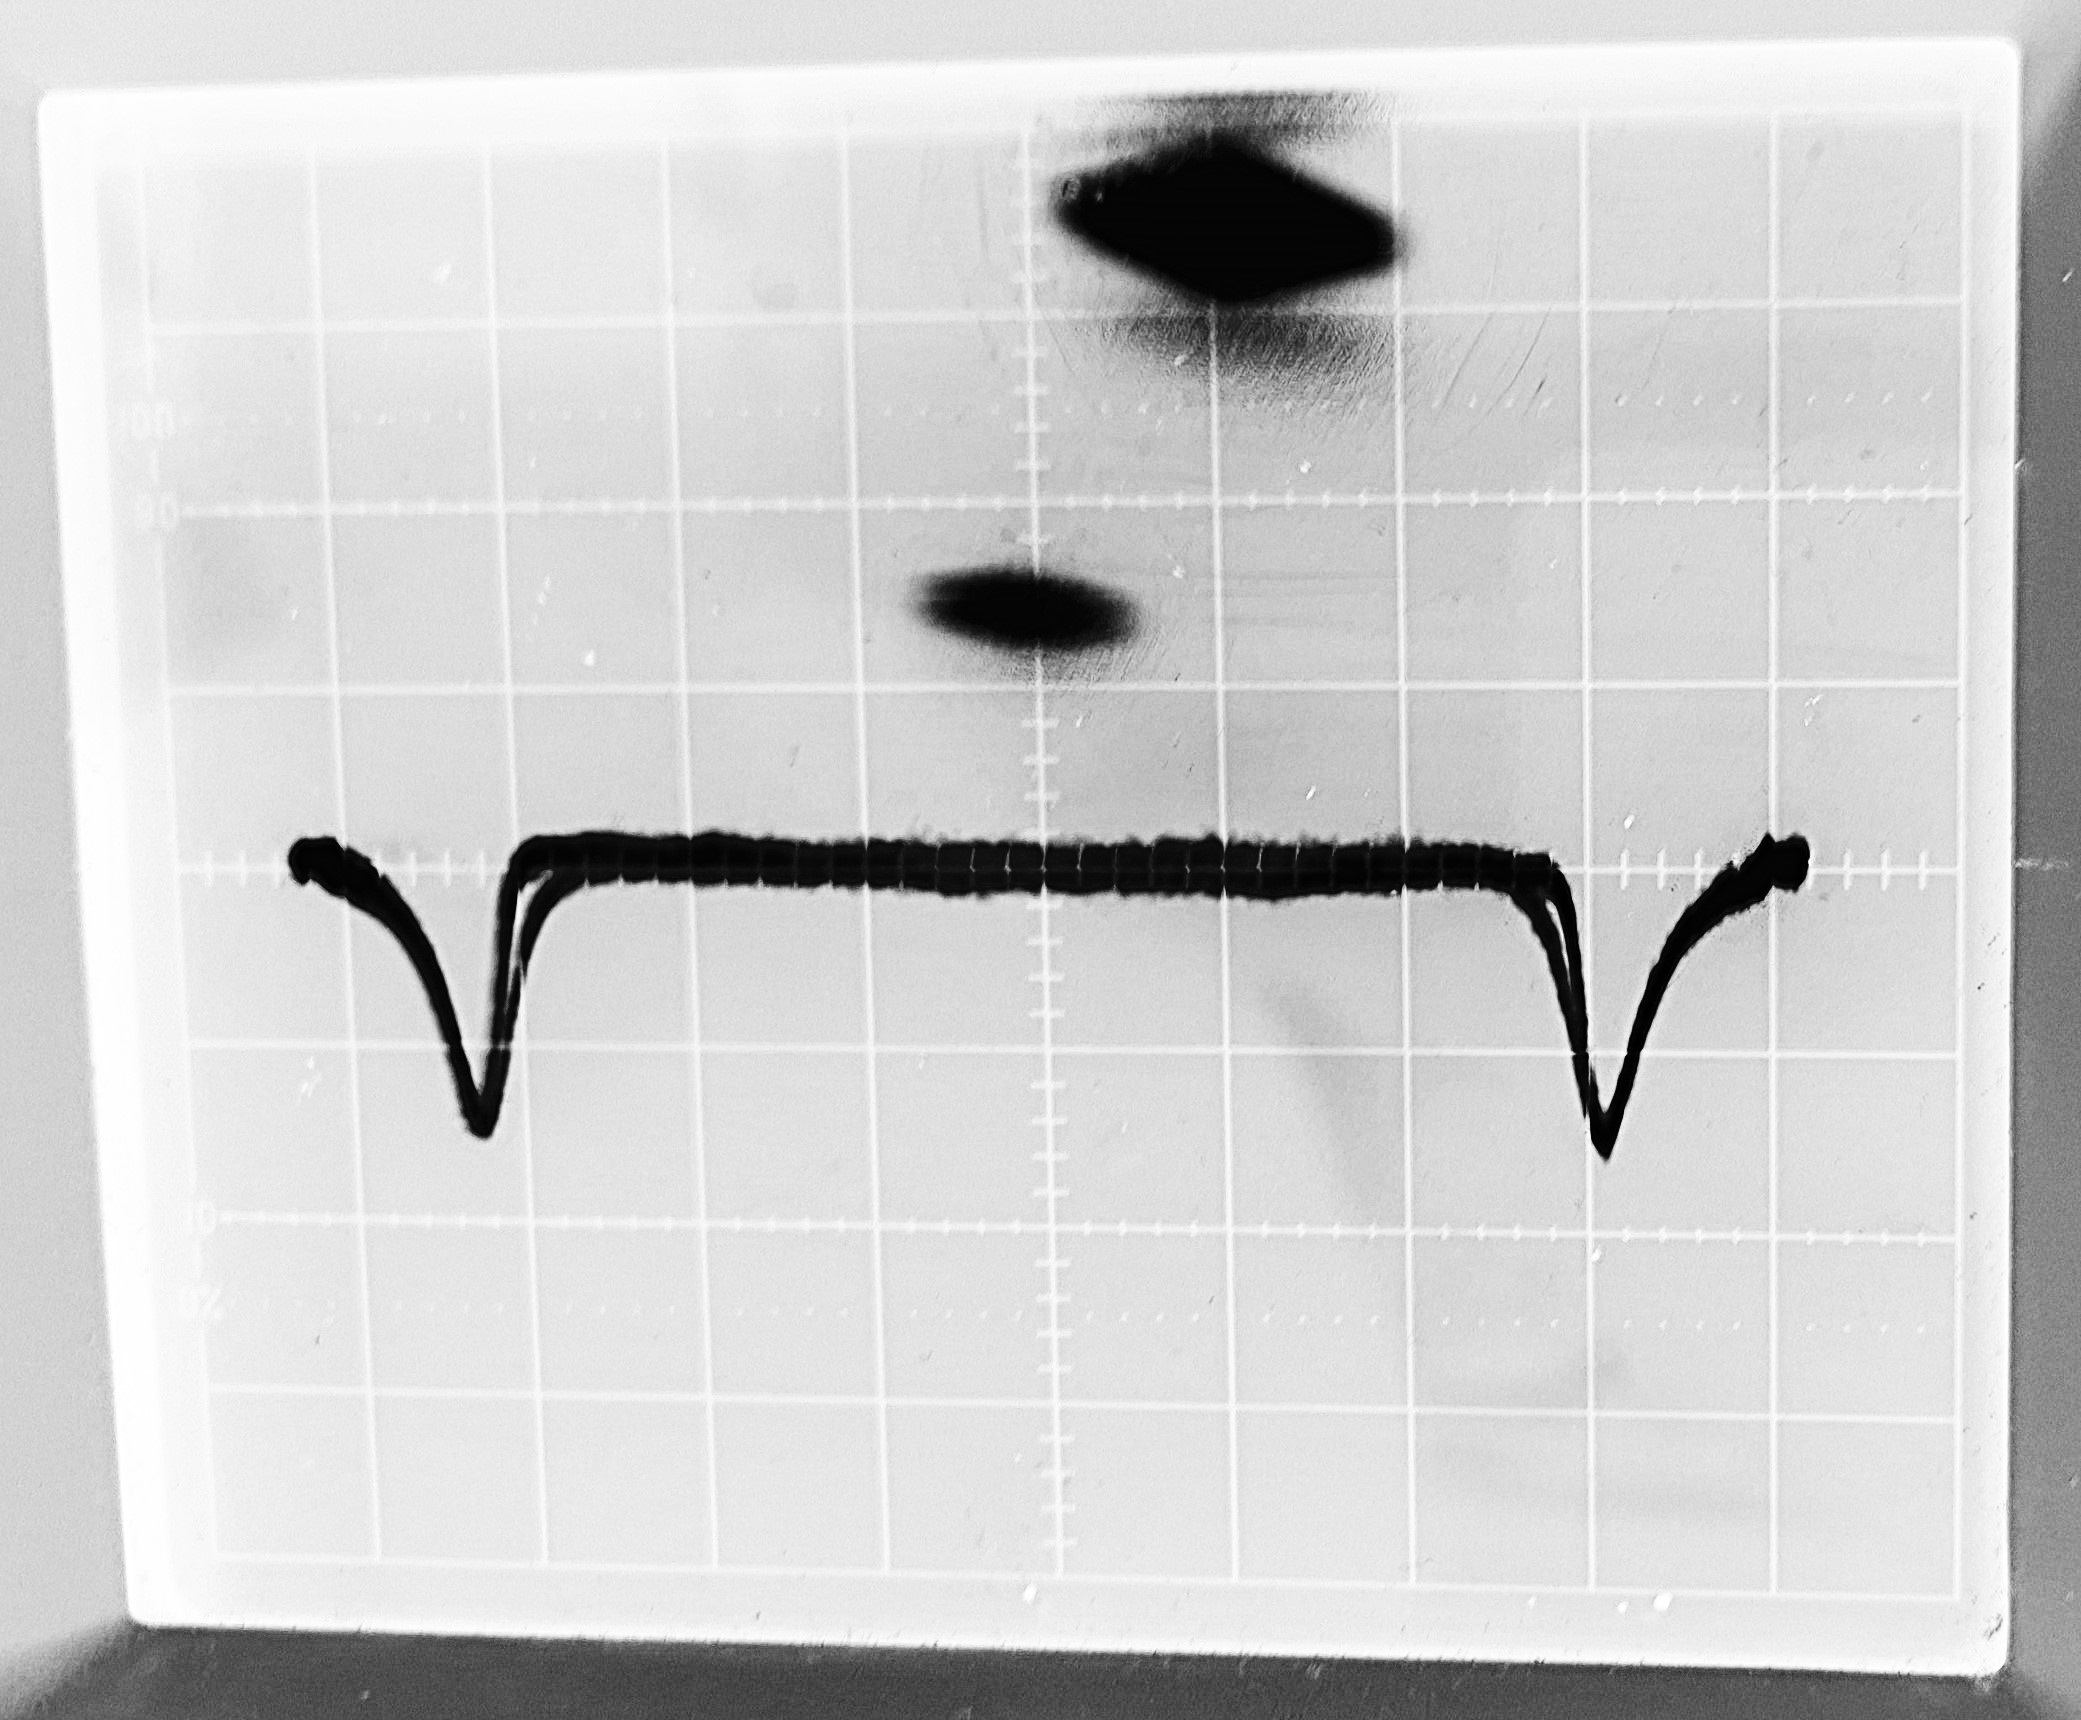
\includegraphics[width=.95\linewidth]{../images/5101-7e}
  \caption{$f=118.34\ МГц$}
\end{subfigure}%
\begin{subfigure}{.5\textwidth}
  \centering
  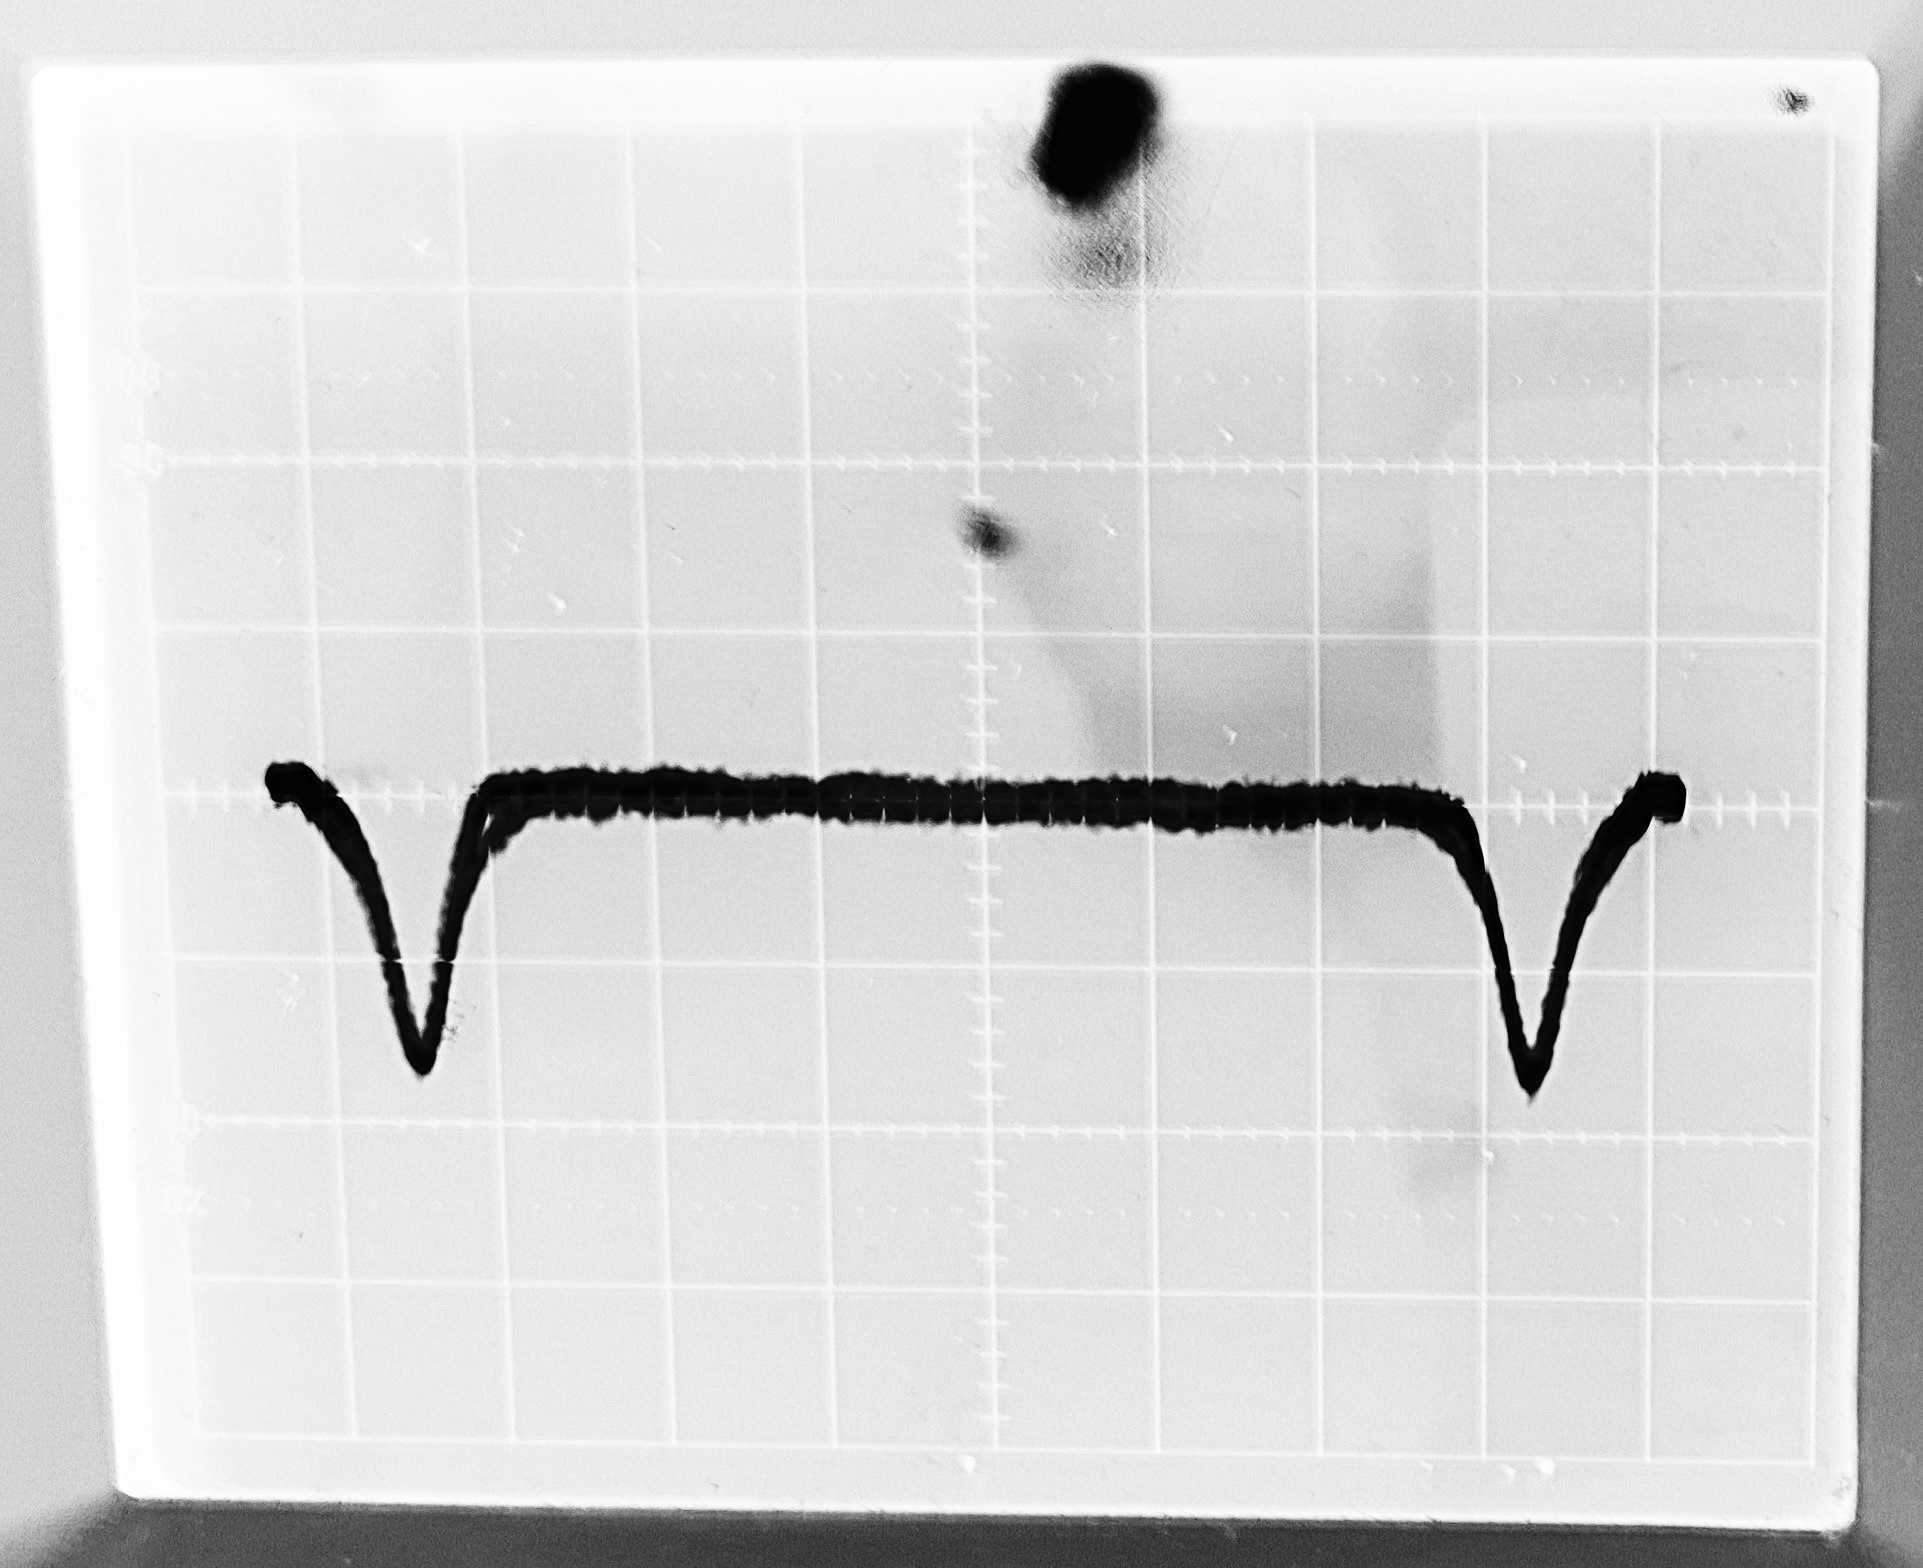
\includegraphics[width=.95\linewidth]{../images/5101-7d}
  \caption{$f=124.34\ МГц$}
\end{subfigure}
\begin{subfigure}{.5\textwidth}
  \centering
  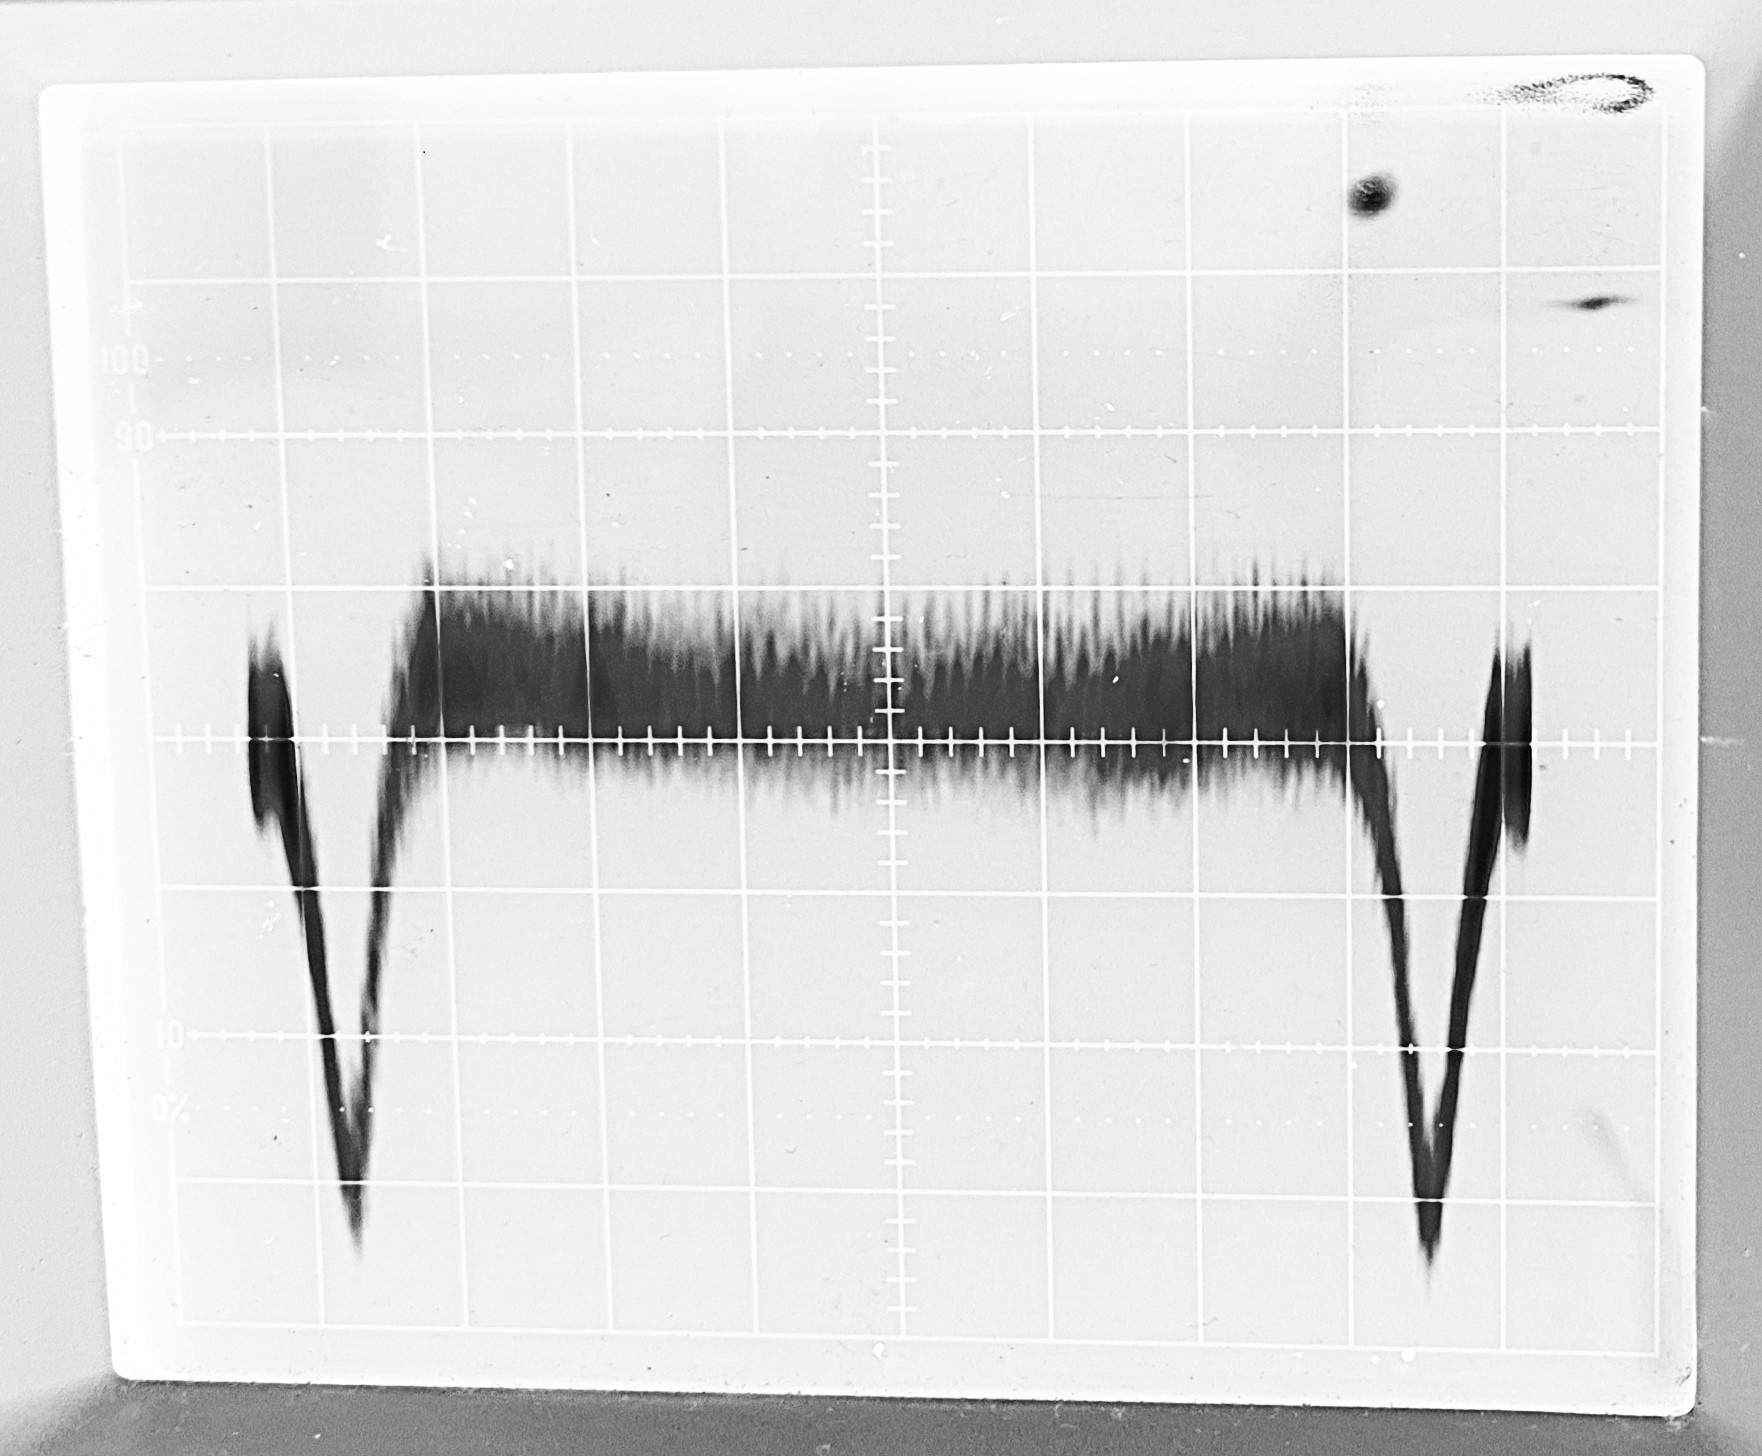
\includegraphics[width=.95\linewidth]{../images/5101-7a}
  \caption{$f=130.34\ МГц$}
\end{subfigure}%
\begin{subfigure}{.5\textwidth}
  \centering
  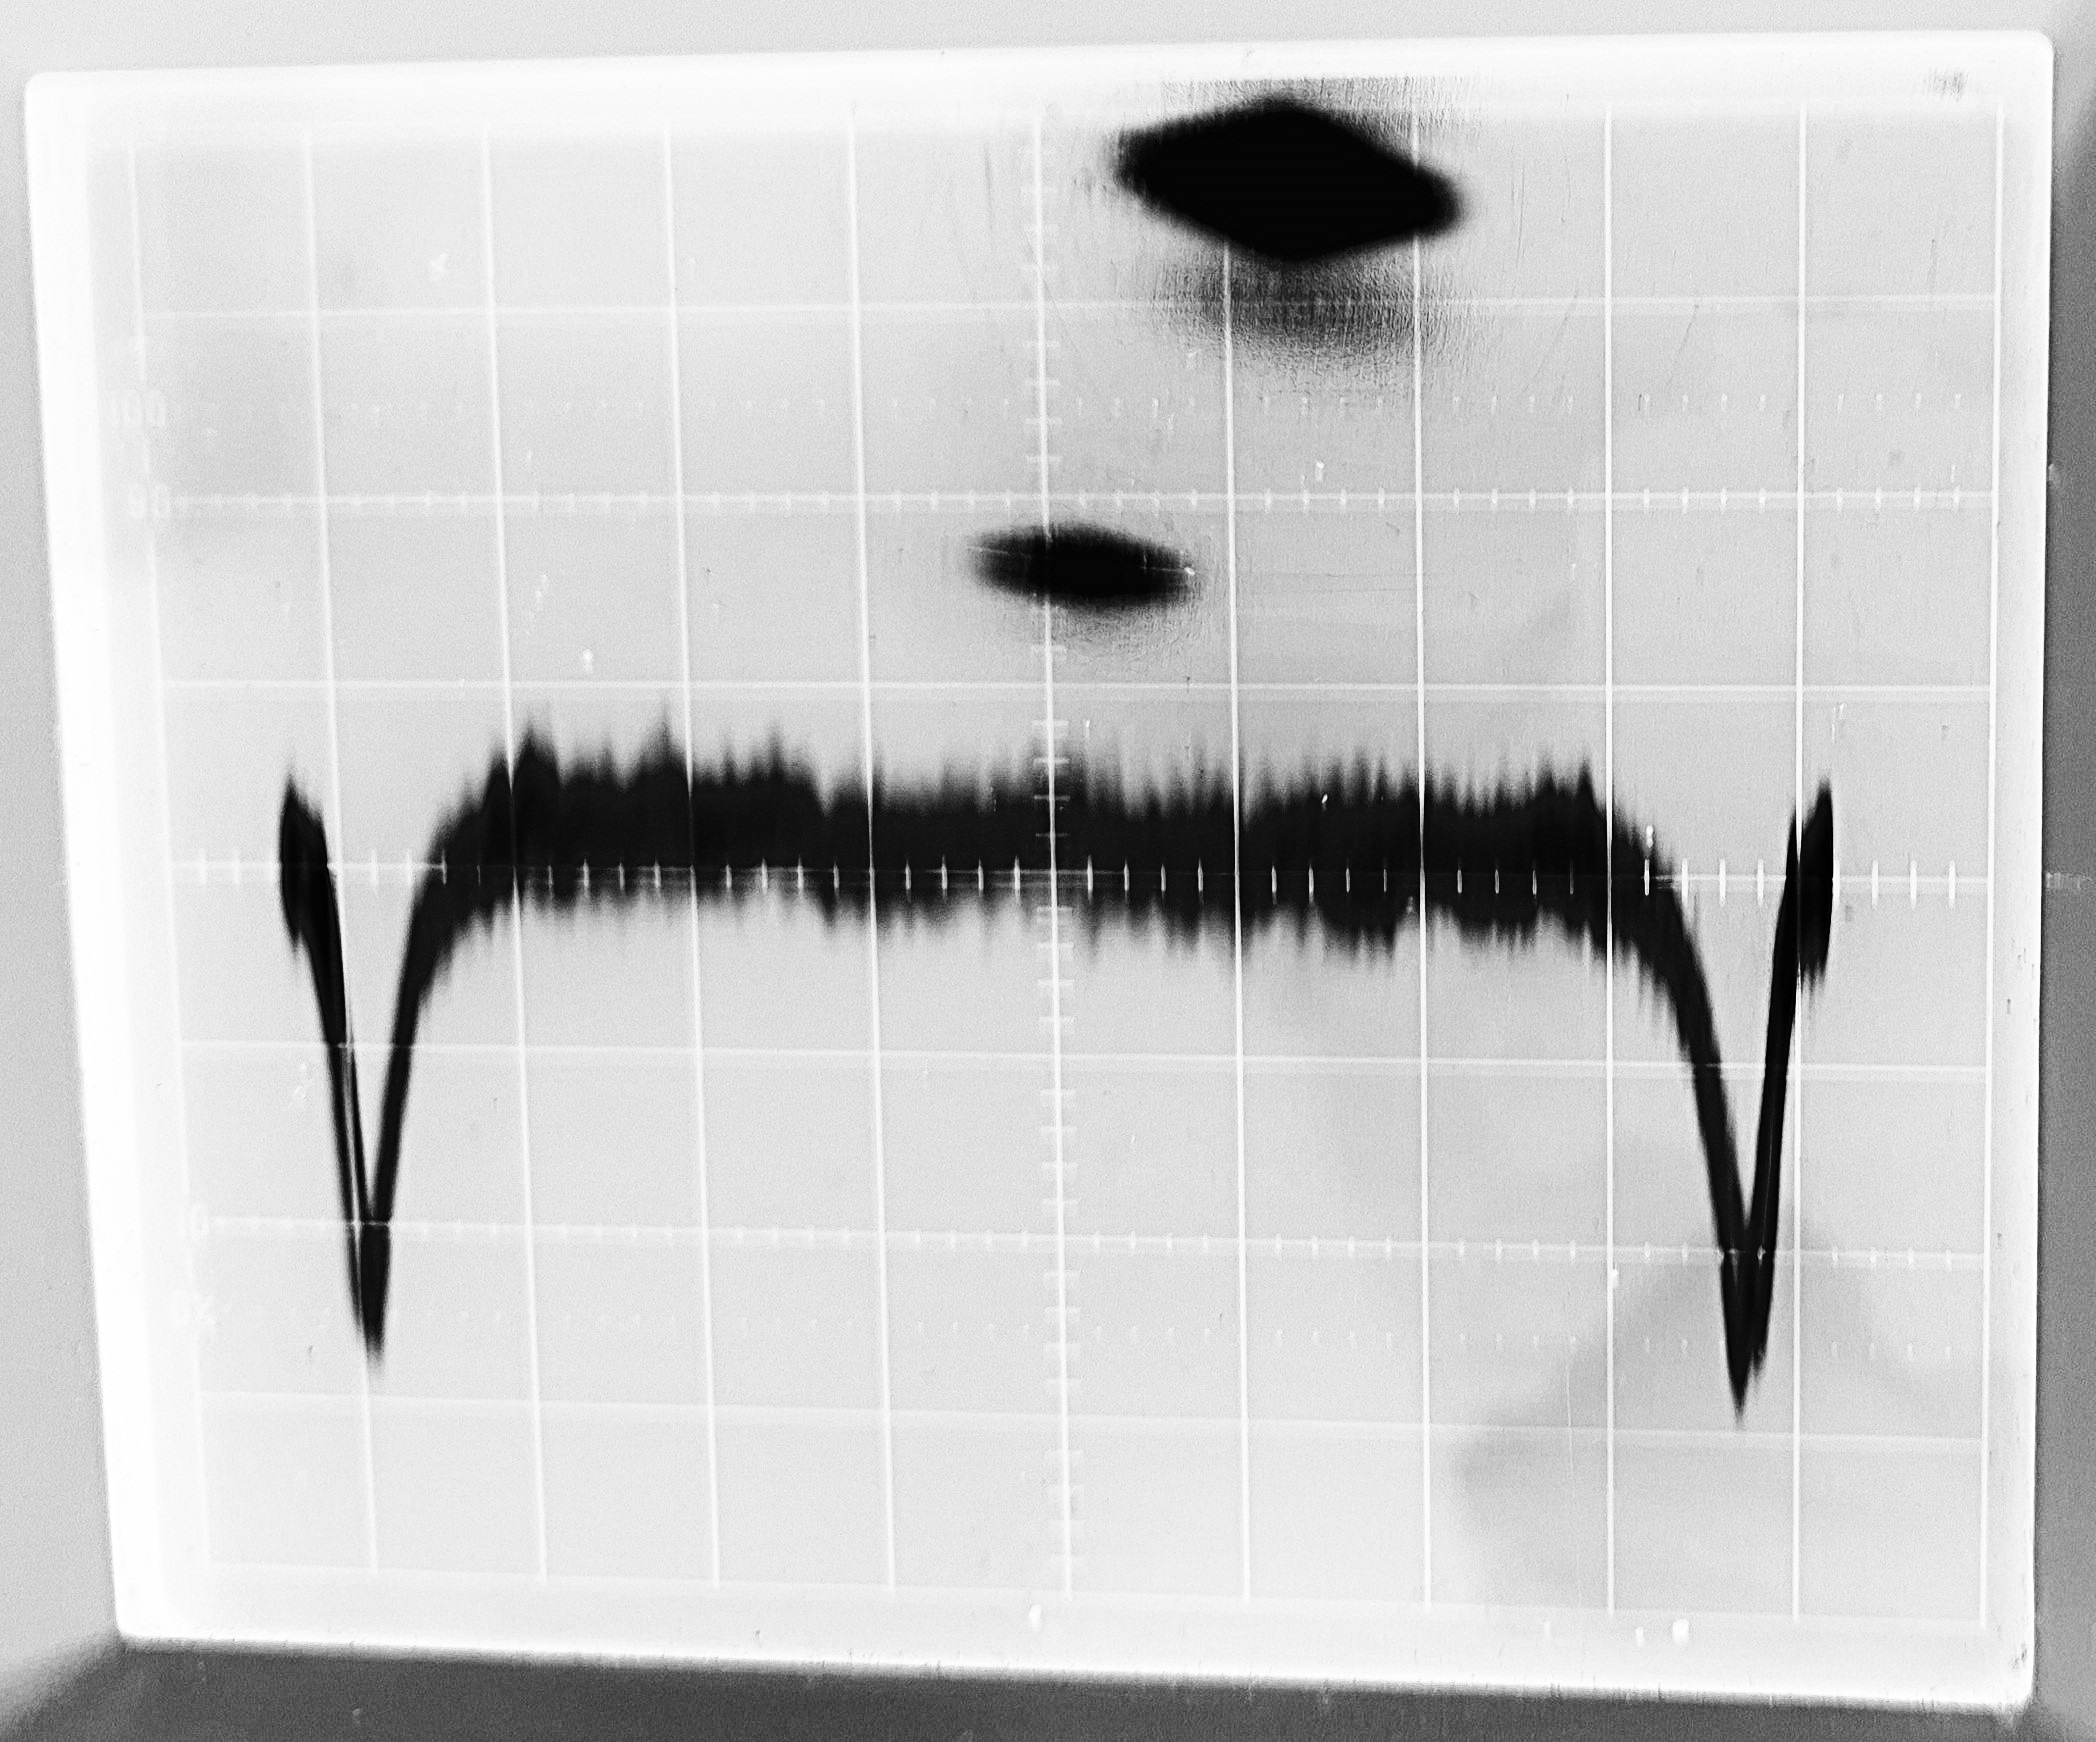
\includegraphics[width=.95\linewidth]{../images/5101-7b}
  \caption{$f=136.34\ МГц$}
\end{subfigure}
\begin{subfigure}{.5\textwidth}
  \centering
  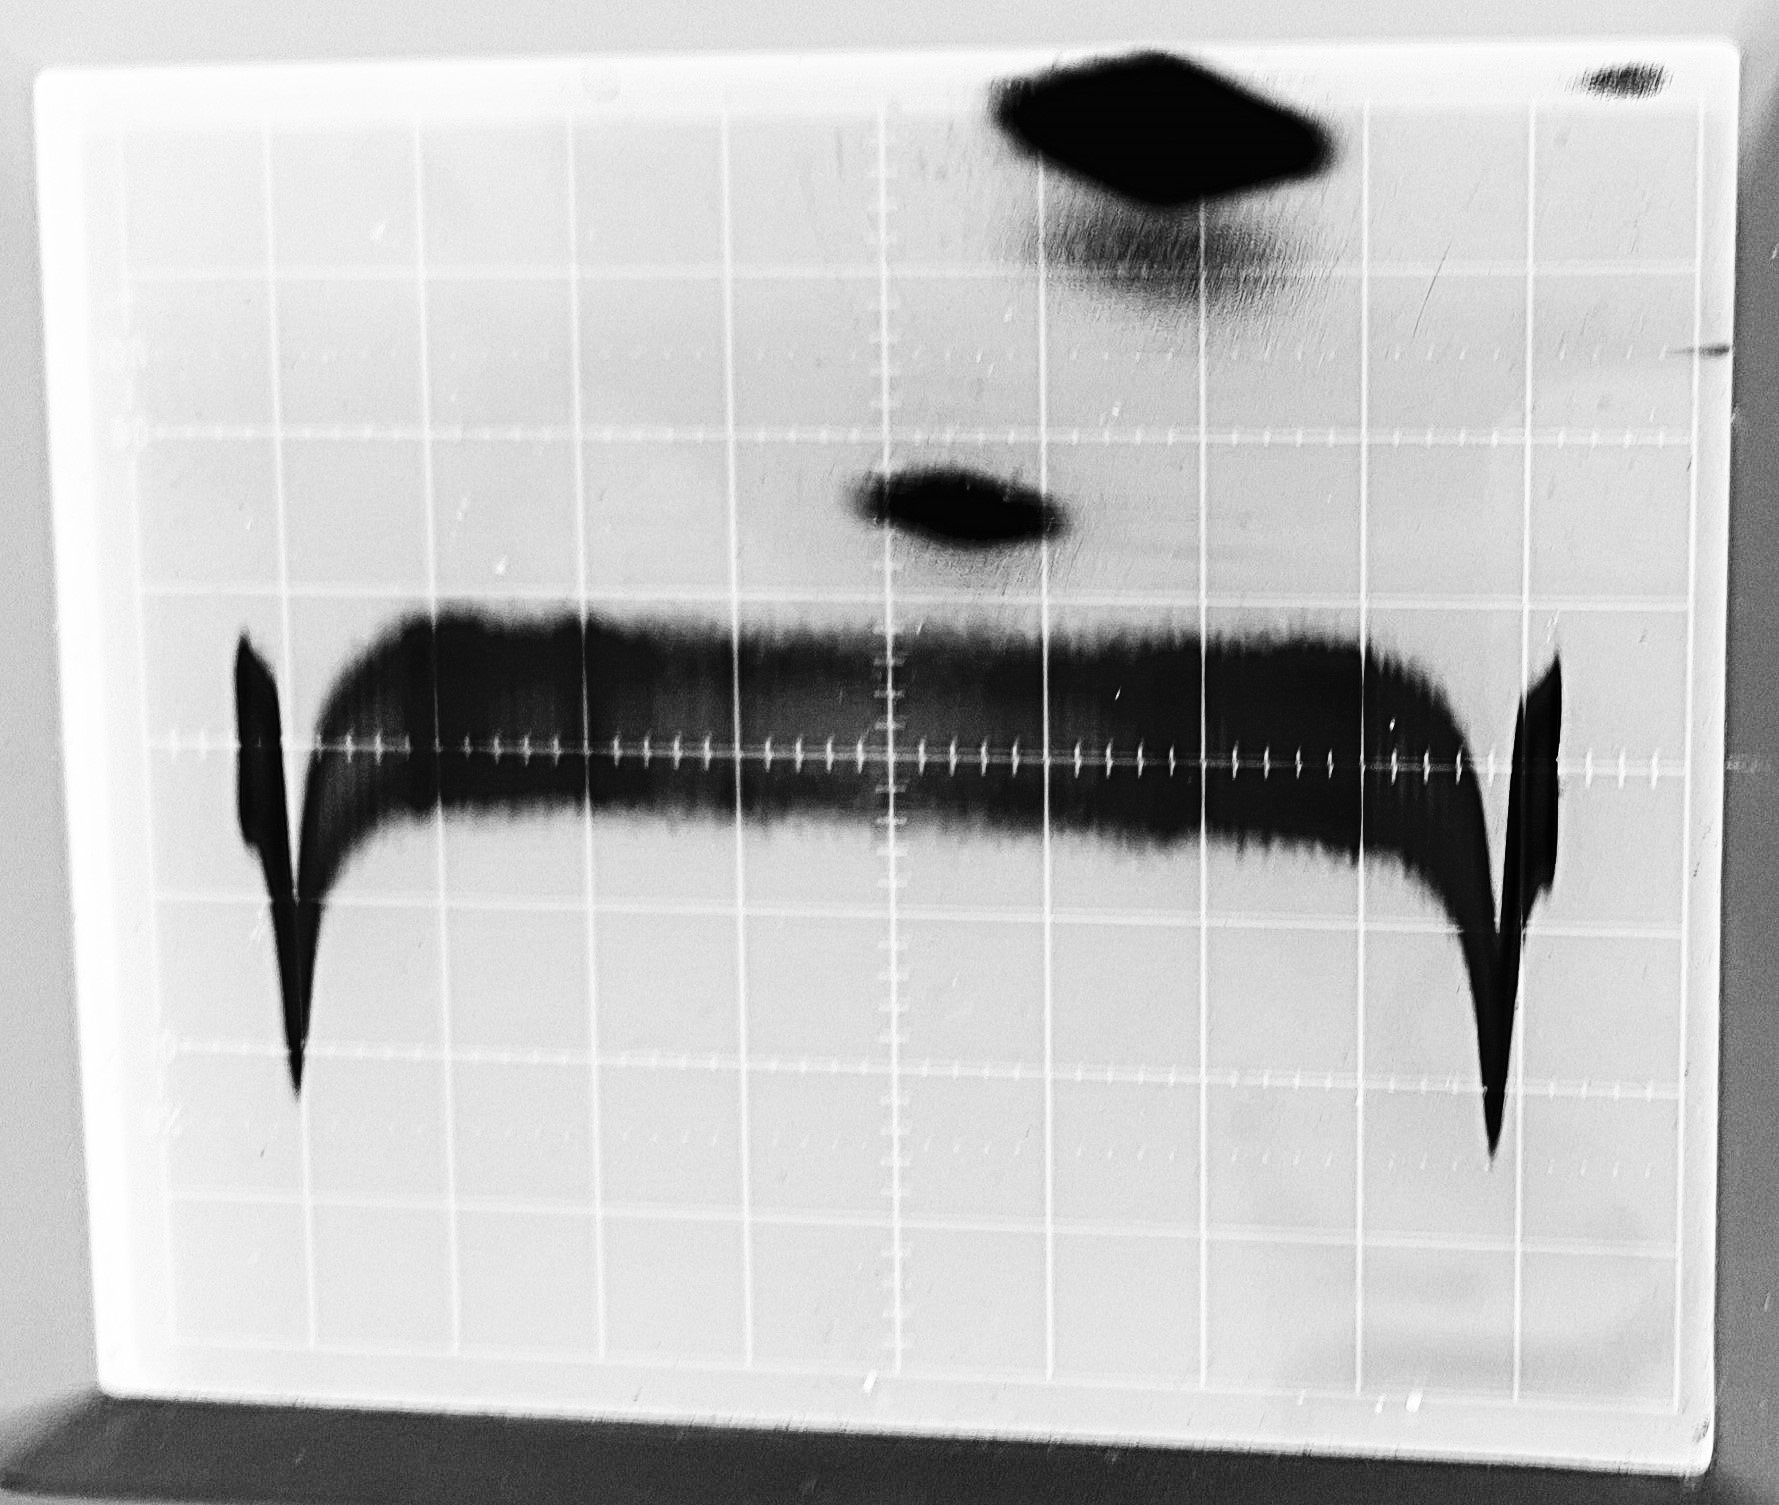
\includegraphics[width=.95\linewidth]{../images/5101-7c}
  \caption{$f=142.34\ МГц$}
\end{subfigure}%
\caption{Картина резонансного поглощения при различных резонансных частотах}
\end{figure}

\item Для каждой из полученных величин определим отношение расстояния между пиками к полной ширине магнитного поля $\eta=B_0/B_{полн}$.
\[\eta_a=0.74\pm0.03, \quad \eta_b=0.78\pm0.04, \quad \eta_c=0.84\pm0.04, \quad \eta_d=0.88\pm0.03, \quad \eta_e=0.91\pm0.04\]

\item Из третьего коэффициента (при резонансной частоте из предыдущего опыта) найдем величину $B_{полн}$.
\[B_{полн}=\frac{B_0}{\eta_c}=(5.7\pm0.4)\ мТл\]

\item Из условия электронного парамагнитного резонанса знаем, что
\[h\nu=g\mu_B B_0=g\mu_B \eta B_{полн}\]

\begin{figure}[H]
\centering
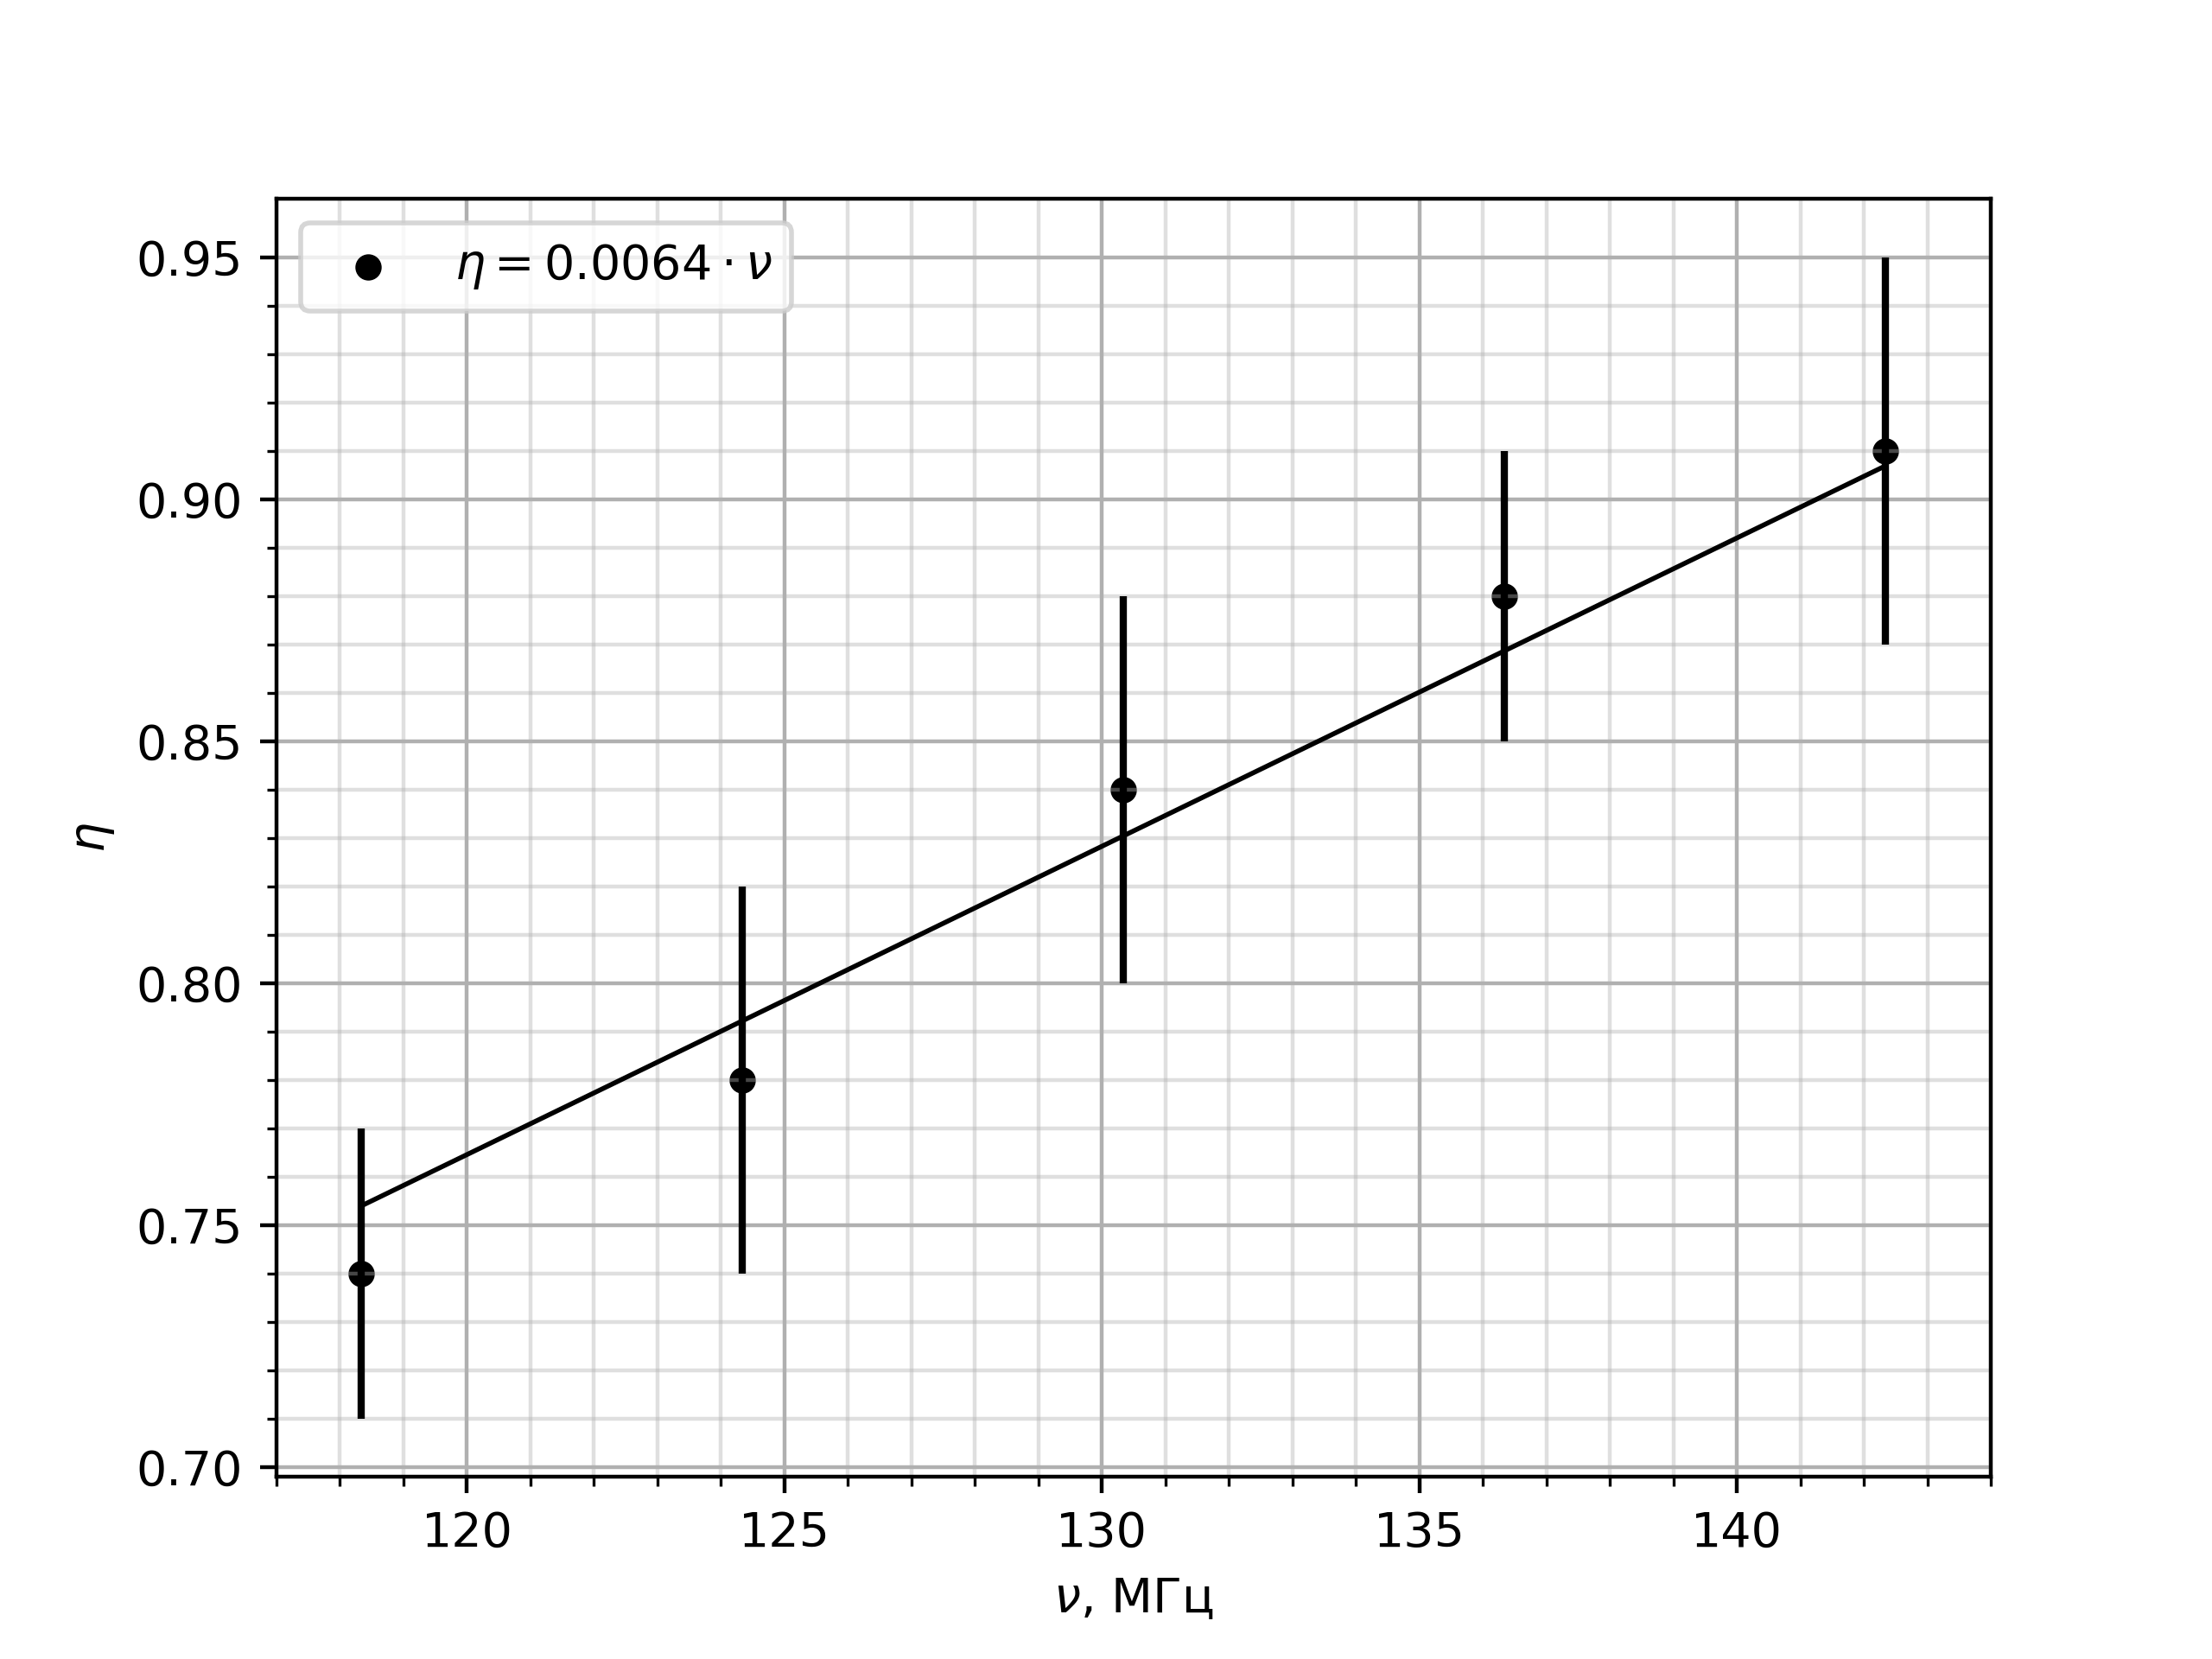
\includegraphics[width=.8\linewidth]{../images/5101-8}
\caption{Зависимость параметра $\eta$ от резонансной частоты $\nu$ колебательного контура}
\end{figure}

\item Вызразим g-фактор из углового коэффициента k проведенной прямой.
\[g=\frac{h\nu}{\eta\mu_B B_{полн}}=\frac{h}{k\mu_B B_{полн}}=1.96\pm0.14\]

\end{enumerate}

Также, дополнительно было проверено, что ширина линии ЭПР не зависит от амплитуды поля в колебательном контуре.

\begin{figure}[H]
\centering
\begin{subfigure}{.33\textwidth}
  \centering
  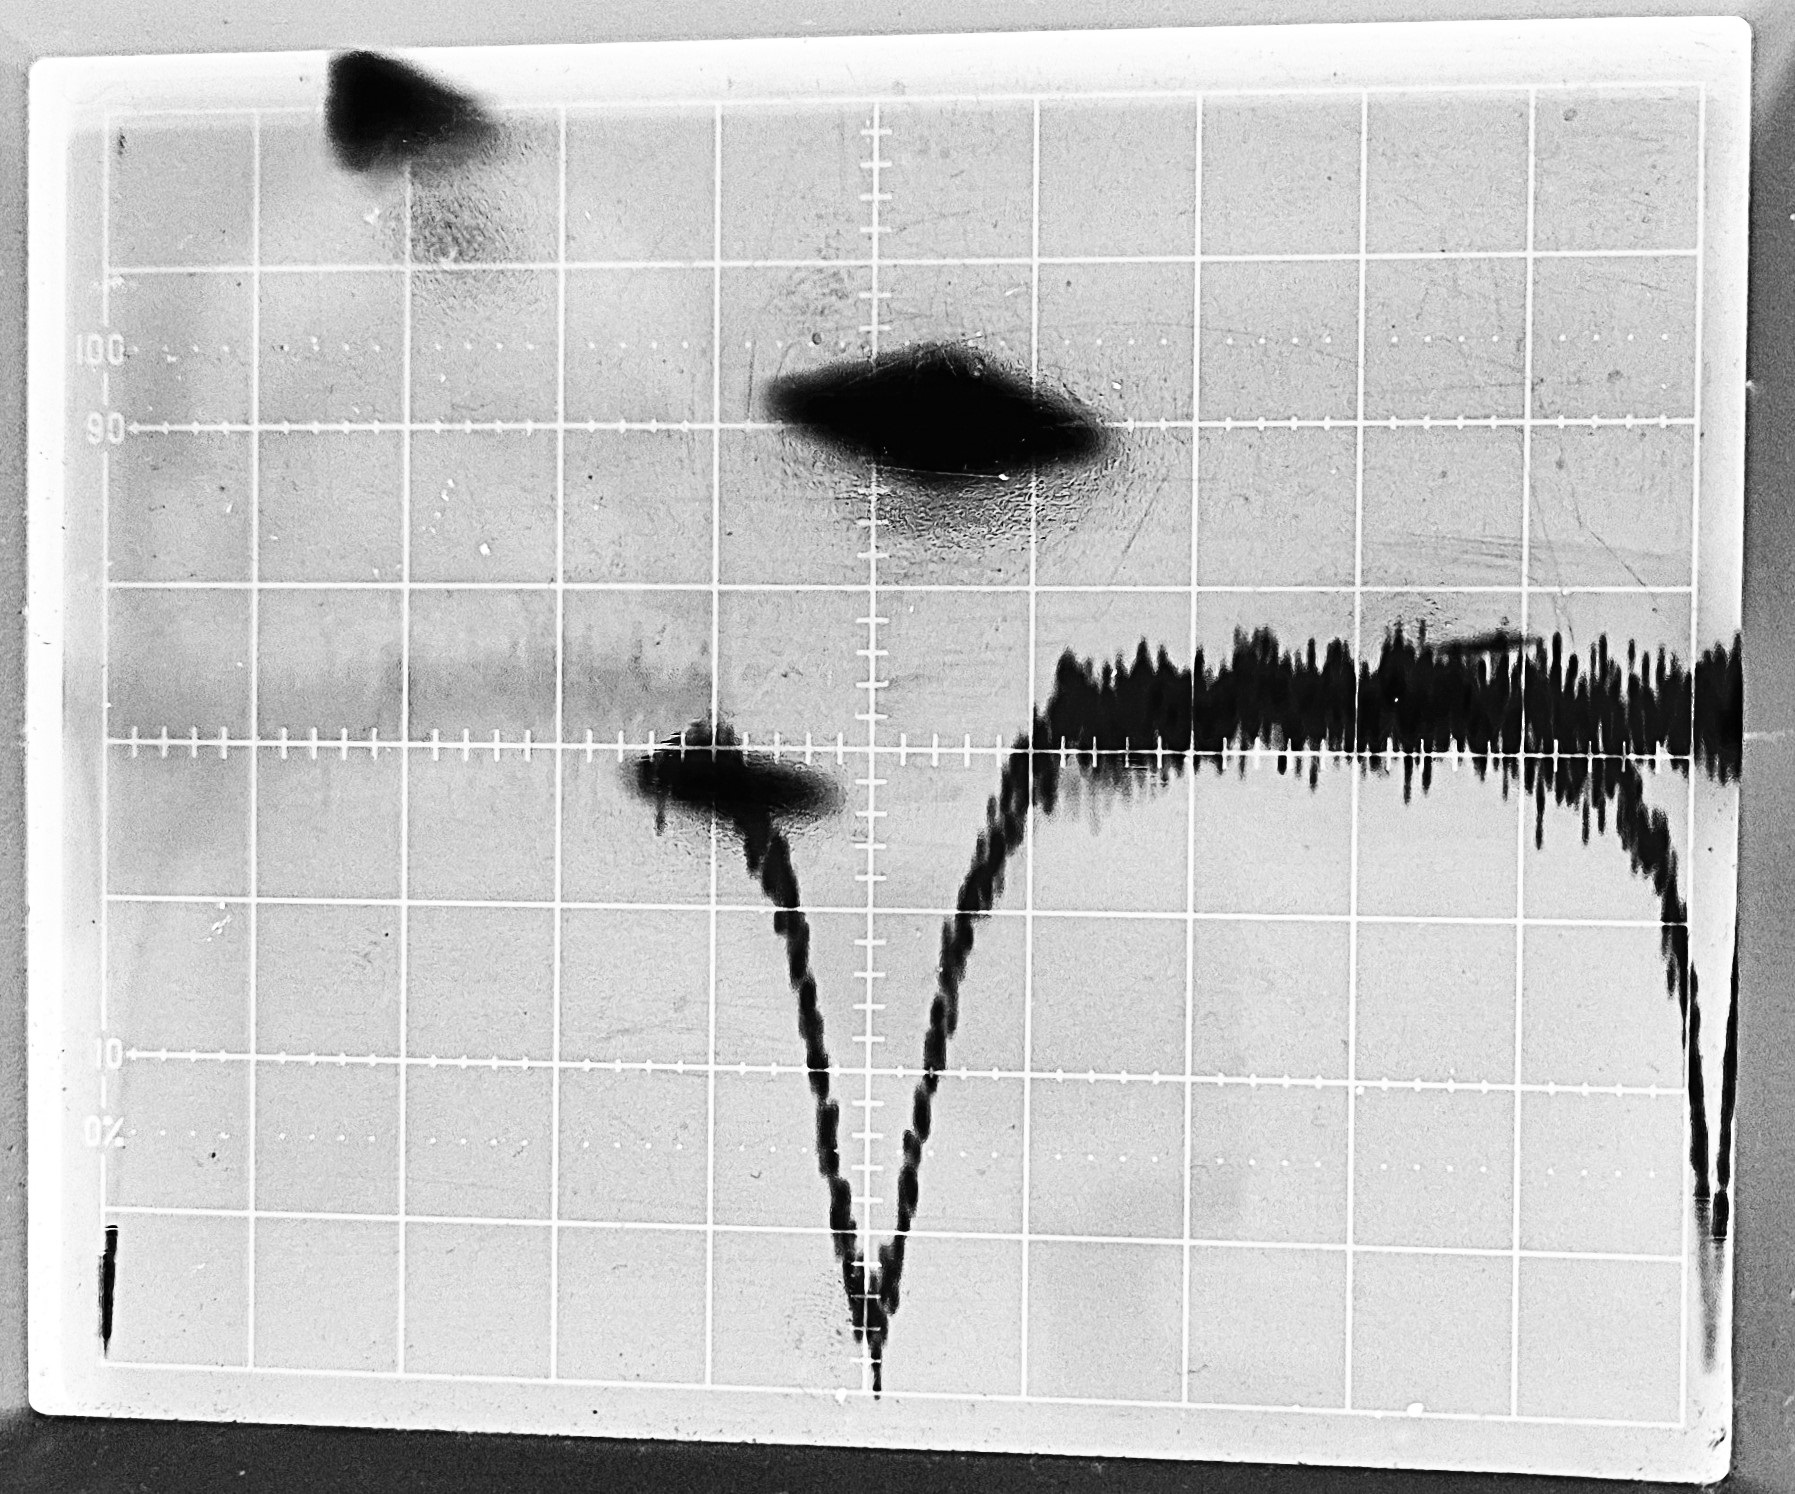
\includegraphics[width=.95\linewidth]{../images/5101-9a}
\end{subfigure}%
\begin{subfigure}{.33\textwidth}
  \centering
  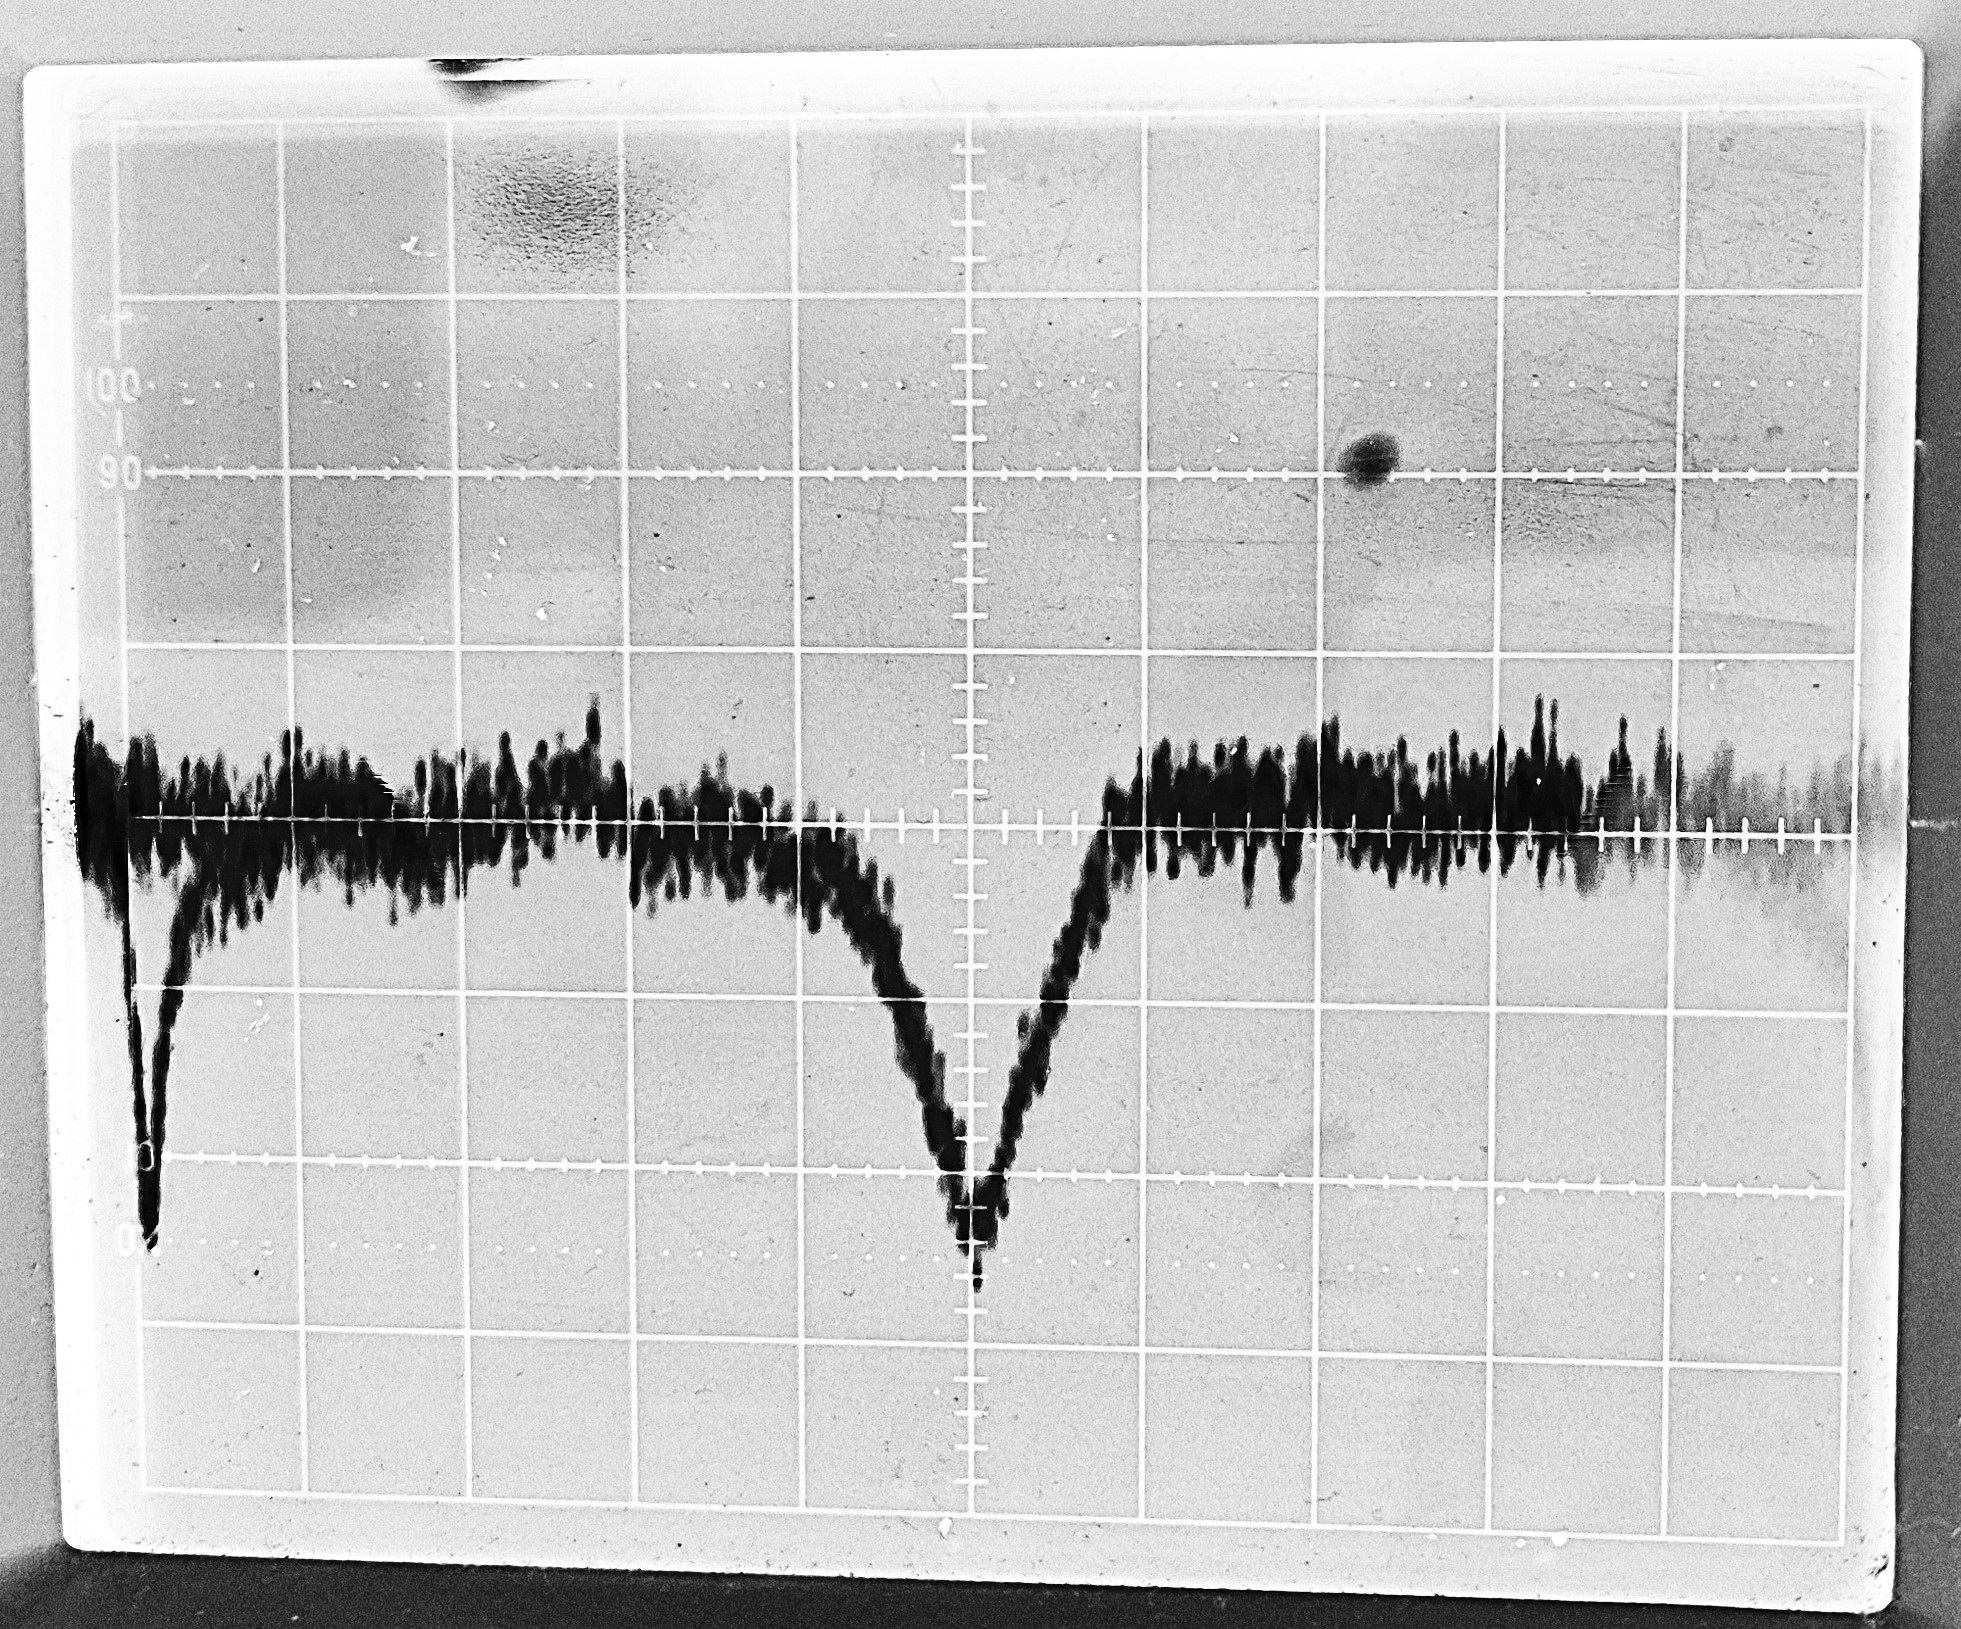
\includegraphics[width=.95\linewidth]{../images/5101-9b}
\end{subfigure}
\begin{subfigure}{.33\textwidth}
  \centering
  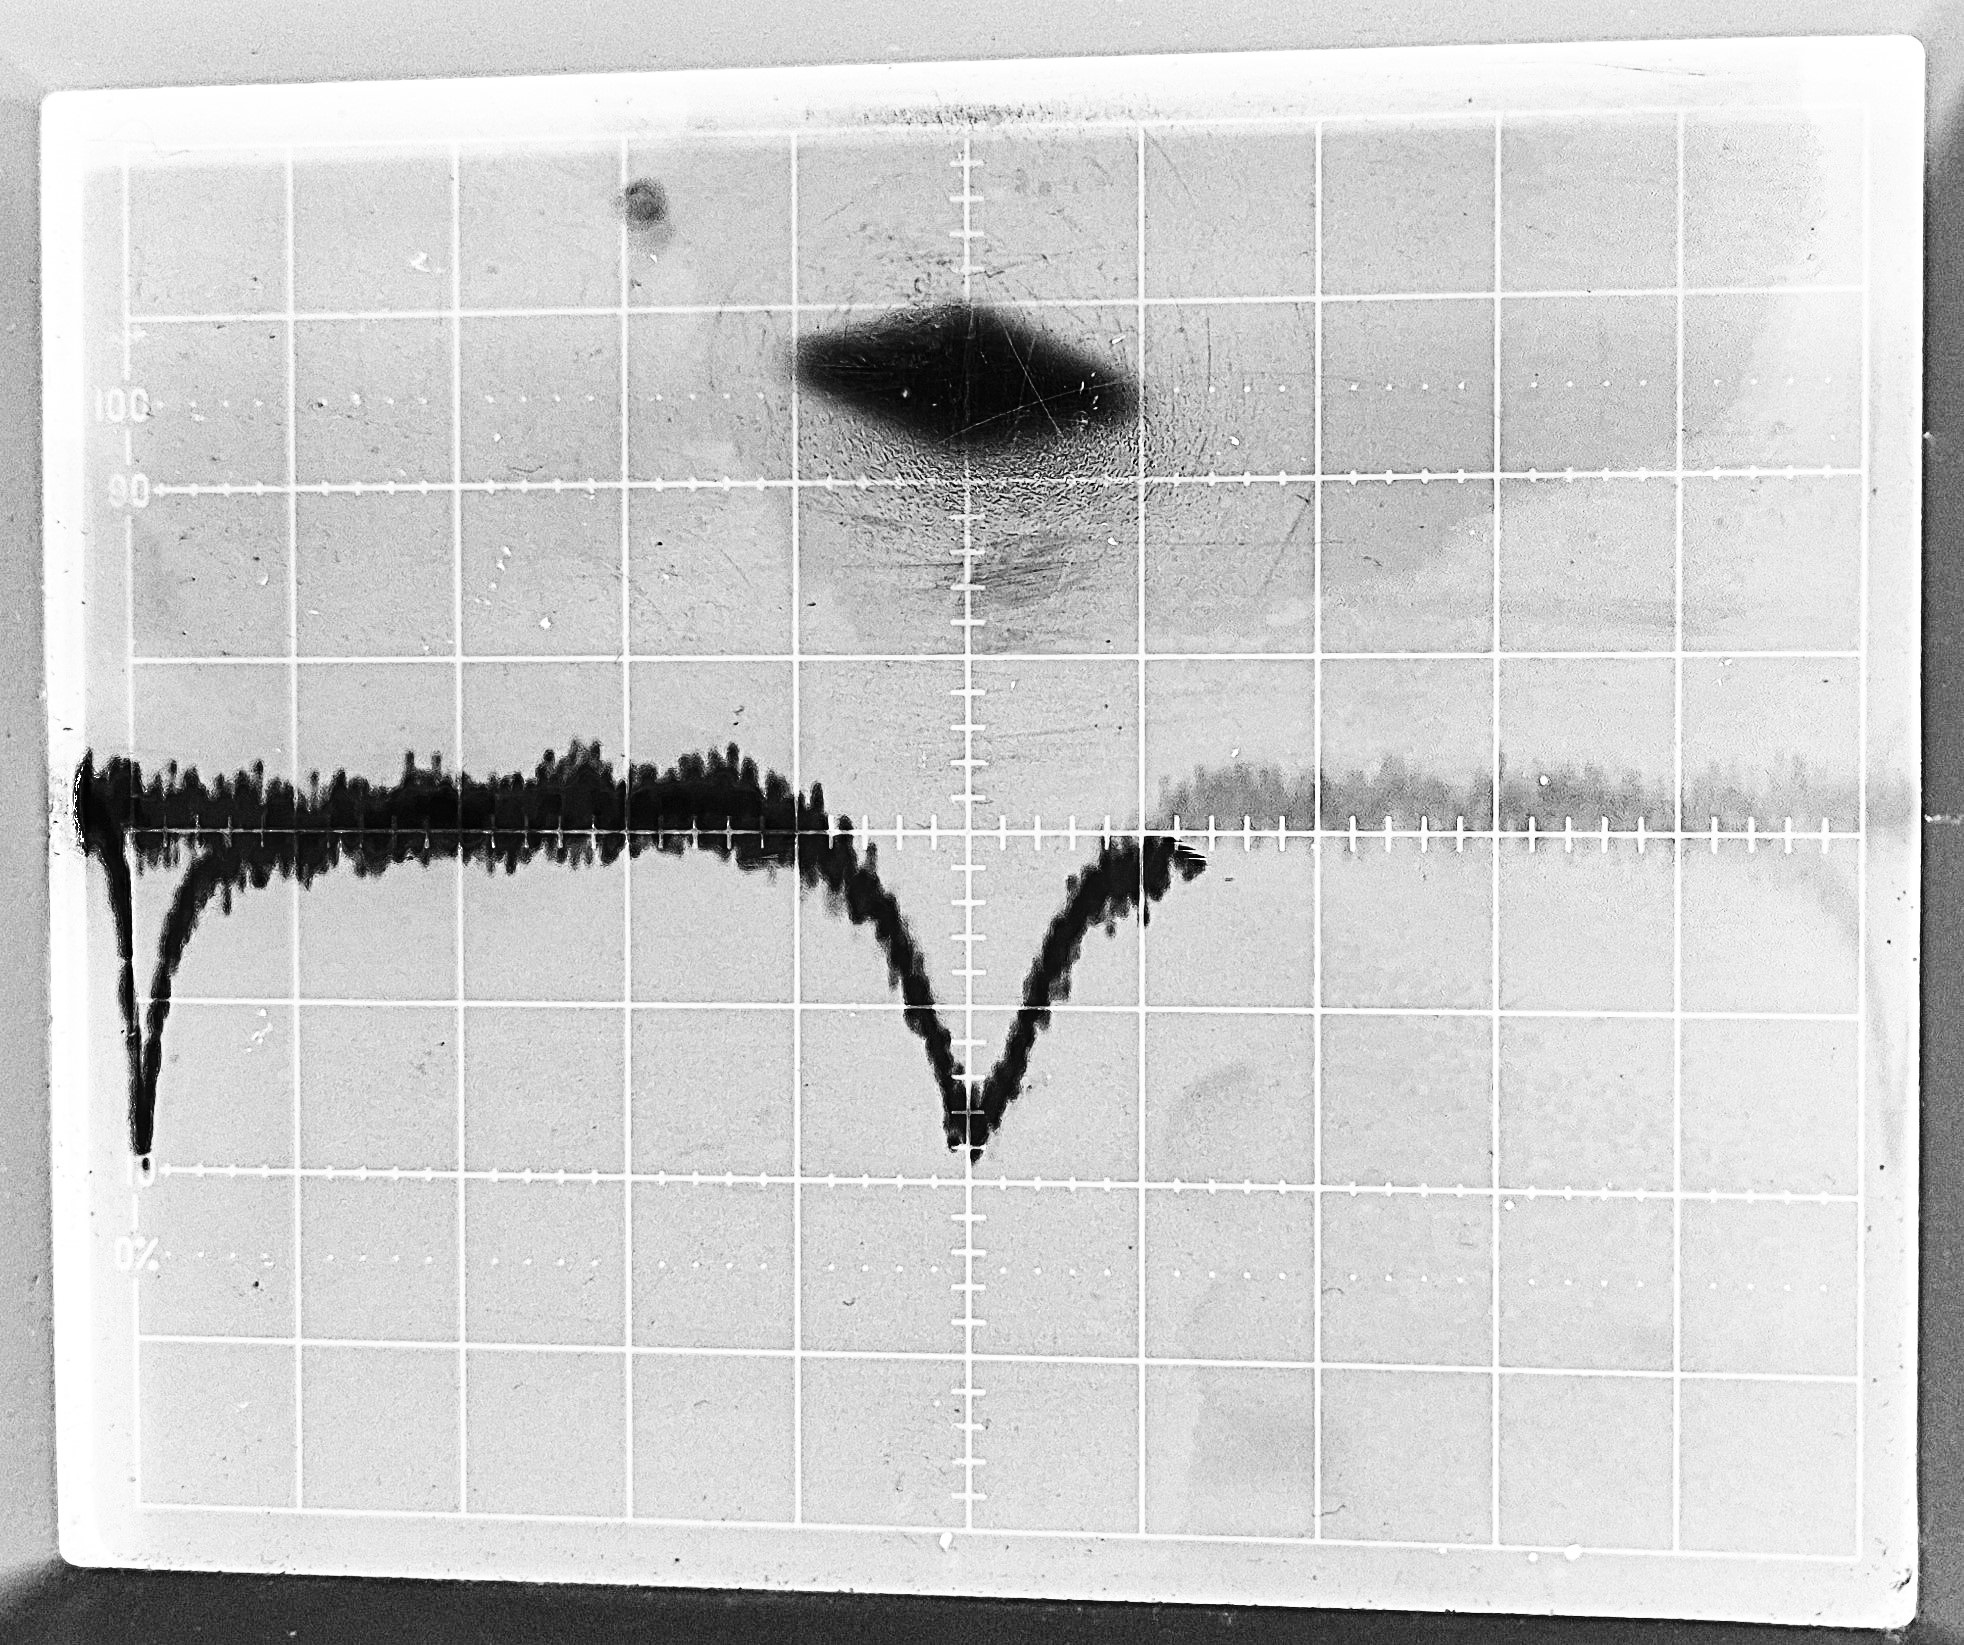
\includegraphics[width=.95\linewidth]{../images/5101-9c}
\end{subfigure}%
\end{figure}

\end{document}